\documentclass[x11names,dvipsnames,svgnames,table,xcdraw]{mmuthesis}
%\newsubfloat{figure}

\usepackage{lipsum}
\usepackage[utf8]{inputenc}
\usepackage[T1]{fontenc}
\usepackage{graphicx}
\usepackage{enumitem}


\usepackage[x11names,dvipsnames,svgnames]{xcolor}
\usepackage[os=win]{menukeys}
\usepackage{listings}

% -------------------------------------------------------------------
% own package
% \usepackage[table,xcdraw]{xcolor}
% -------------------------------------------------------------------

\lstset{language=[LaTeX]TeX,columns=fullflexible,
basicstyle=\ttfamily,texcsstyle=*\bfseries\color{NavyBlue},
commentstyle=\itshape\color{PaleVioletRed4},
frame=single,framesep=6pt,
framexleftmargin=6pt,framexrightmargin=6pt,
xleftmargin=12pt,xrightmargin=12pt,
breaklines=true,breakatwhitespace=true}


% -------------------------------------------------------------------
% user annotations
% -------------------------------------------------------------------

% \begin{comment}
\newcommand{\ian}[1]{\textcolor{red}{#1}}
\newcommand{\lk}[1]{\textcolor{blue}{#1}}
\newcommand{\js}[1]{\textcolor{magenta}{#1}}
\newcommand{\cc}[1]{\textcolor{teal}{#1}}
\newcommand{\rl}[1]{\textcolor{green}{#1}}
% \end{comment}

\begin{comment}
\newcommand{\ian}[1]{}   % turn off
\newcommand{\lk}[1]{}   % turn off
\newcommand{\js}[1]{}   % turn off
\newcommand{\cc}[1]{}   % turn off
\newcommand{\rl}[1]{}   % turn off
\end{comment}


\newcommand*\mean[1]{\bar{#1}}
\newcommand{\versionOne}{LSH-Inspired Semantic Extraction and Retrieval Engine (Version 1) }
\newcommand{\versionTwo}{Chamfer Distance based Semantic Extraction and Retrieval Engine (Version 2) }




% -------------------------------------------------------------------
% own packages
% -------------------------------------------------------------------
\usepackage{amssymb}
\usepackage{multirow}



\author{Clarence Cheong Weihan}
\title{Large Scale Extraction and Retrieval of Video Semantics for Carpark Surveillance Videos}
\submissionyear{2018}
\submissionmonth{August}
\faculty{Faculty of Computing and Informatics}
\degree{Master~of~Science (Information~Technology)}
\qualification{B.Eng.~(Hons), Multimedia University, Malaysia\\%
}

% load acronym definitions from separate file
\loadglsentries{myacronyms}

\begin{document}

\frontmatter
\makecoverandtitlepage
\copyrightpage
\declarationpage

\acknowledgements{
Firstly, I would like to thank my wife, Jocelyn for encouraging me to take on this seemingly "less traveled road". Her unceasing support and understanding throughout this journey is precious and much appreciated. 

Undeniably, this journey would not be possible without the advices, ideas and guidance provided by my supervisors, Dr. John See as well as Dr. Wong Lai Kuan. Their input certainly has sparked ideas which has been materialized in this work. Thanks you, I owe you many.

Not forgetting my family and friends who supported me on this journey. My fellow church members who were encouraging me throughout my masters. Thanks a lot! 

Last and not least, I would like to applaud myself and give myself some credit for putting myself out there, not being afraid to chase after goals and take on challenges that I would have never thought of. 
}
\dedication{To my parents, my wife, and my family.}

\abstractfromfile{abstract}

{\clearpage\SingleSpacing
\tableofcontents\clearpage
\listoftables\clearpage
\listoffigures\clearpage}

\prefacefromfile{preface}

\mainmatter

\chapter{Introduction}
The use of video based surveillance system has exploded over the past decade. The ease of implementation along with its benefits drew the attention of both the public and private sectors, without a doubt, the digital security industry caught on to it and consequently bloomed with more and more retail stores, shopping malls, and even homes equipping themselves with closed circuit televisions (CCTV) as a means for safety precaution. With the rise of such technology and coupled the hype around the idea of Internet of Things (IoT) and Big Data over the recent years, there has been a deeper thirst among researchers in finding ways for practical uses of bridging existing data with technology to bring about a new wave in the research field.

\subsection{Overview}
\label{section:introduction}
%In this work, the author takes on a journey to explore this new research territory of utilizing video based surveillance footage for 

Traditionally, the process of finding a particular video from a huge collection is done manually. This process involves an inquirer who is looking for a particular scene or shot, and an person-in-charge who manages the CCTV video collection. In a carpark scenario, the inquirer would typically need to provide information such as time, date, color of the vehicle, vehicle registration number, and place of which an incident occurred. 

Next, the person-in-charge would have to sift through hours and hours of video in order to find a distinct video shot. This process is undeniably time consuming, laborious, monotonous and tedious. While the task is potentially simpler and straightforward when there is only one video shot with clear-cut definitive time and date given, this process takes an enormous effort when the time and date is not given, or even in cases when all the video shots with similar properties are desired. 

Evidently, there exist a gap which can be addressed using a well designed retrieval engine.


\subsection{Motivation and Problem Statements}

\subsection{Research Objectives}




\subsection{Scope of Thesis}
\label{subsec:scope}
\cc{** explain what semantic is, what type of semantic we are trying to extract and the scope of the work} 



\subsection{Contribution}

\subsection{Organization of Thesis}
%!TEX root=thesis.tex
%This is the draft literature review. 

%!TEX ROOT = thesis.tex


\chapter{Background Studies}
\label{section:litreview}

In this chapter, related theoretical background concepts are first introduced. Then, the related works are discussed in two main portions: 
\begin{enumerate}
    \item Existing methodology and techniques used for semantics extraction
    \item Recent methodology and techniques used for semantic retrieval.
\end{enumerate}



\section{Related Theoretical Background Concepts}
\label{subsec:relatedConcepts}

Before diving deeper into the nitty-gritty of the proposed framework, fundamental understanding towards related theoretical background concepts used in this work is discussed. As this work covers a rather broad spectrum of different concepts, a general understanding towards these concepts would provide some degree of clarity towards the topic at hand. This section briefly describes the fundamental of the following concepts: i) Quantization, ii) Distance Measure, iii) Human Visual System, \& iv) colour Model and colour Terms. 


\subsection{Quantization}

The use of quantization in the mathematical and digital signal processing field is not a new concept. Digital signal processors are limited by natural boundaries such as hardware limitations, and are only able to compute and perform arithmetic operations within a limited range \cite{spors_2018}. The use of quantization refers to the process of mapping and projecting a set of large values which are often continuous or analog in nature into a set of discrete and finite values. 

\begin{figure}[hbt!]\centering
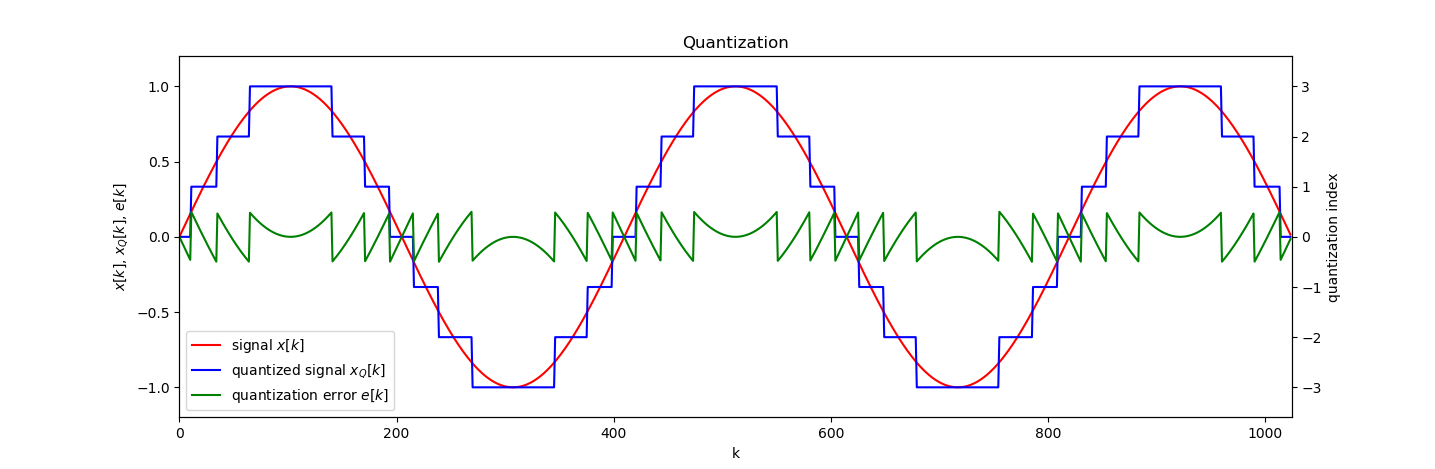
\includegraphics[width=\textwidth]{image/general/quantization.png}
\caption{Quantization}
\label{fig:quantize}
\end{figure}


The use of quantization enables reduction in memory usage (compression) as well as the reduction of computational cost, hence, leading to faster processing speed. However, since the quantization process is a many-to-few mapping operation, the operation is considered irreversible without prior knowledge of the loss. Nevertheless, the output discrete signal can closely resemble the continuous input signal depending on the number of quantization level used.
\begin{equation}\centering
\label{eq:quantization}
x_Q[k] = g( \mspace{3mu}\lfloor \mspace{3mu}f(x[k]) \mspace{3mu}\rfloor\mspace{3mu})
\end{equation} 
\vspace{-3em}
\begin{equation}\centering
\label{eq:quantizationerror}
e[k] = x_Q[k] - x[k]
\end{equation}
In order to expound on the quantization process, a mathematical model of this process can be formulated as such. Consider a continuous signal $x[k]$ whose quantized signal, $x_Q[k]$, is desired (see Equation \ref{eq:quantization}). The functions $f (\mspace{3mu} \cdot  \mspace{3mu})$ \& $g (\mspace{3mu} \cdot  \mspace{3mu})$ can be thought of as a real-value mapping function while the $\lfloor \mspace{3mu} \cdot  \mspace{3mu} \rfloor$ represents a rounding function. The $f (\mspace{3mu} \cdot  \mspace{3mu})$ function is used to convert real-world values into a digital signal, while $g (\mspace{3mu} \cdot  \mspace{3mu})$ is used to map the digital signal into a quantized signal. As previously mention, this process is considered irreversible with prior knowledge of the loss, in this case, the quantization error, $e[k]$, can be computed as Equation \ref{eq:quantizationerror}. Figure \ref{fig:quantize} illustrates a quantization process where the red signal ($x[k]$) represents the real-world continuous signal, the blue signal ($x_Q[k]$) refers to the quantized signal while the green signal ($e[k]$) represents the error due to quantization process.

In order to leverage on this concept, in this work, the quantization technique was extended further into a three dimensional space. As video data can be represented in a 3D space, the quantization process was used to quantize the continuous video data into a set of discrete and finite values. These discrete and finite values can ease the calculation and manipulation of data. As colour space can also be represented using a 3D space, this concept was adapted and applied here to quantize the colour space into colour terms (See Section \ref{section:colourterm}).



\subsection{Distance Measure}
\label{section:distancemeasures}

The use of distance measure is another recurring key concept in the proposed method. Given that distance measures are commonly used in computer science as well as the mathematics field, there are numerous metrics suggested by different authors which are applicable and useful in different scenarios. In essence, distance measure is used to compute the difference between targets. On the flip side, the difference can also be thought of as the similarity between these targets.

\begin{figure}[hbt!]\centering
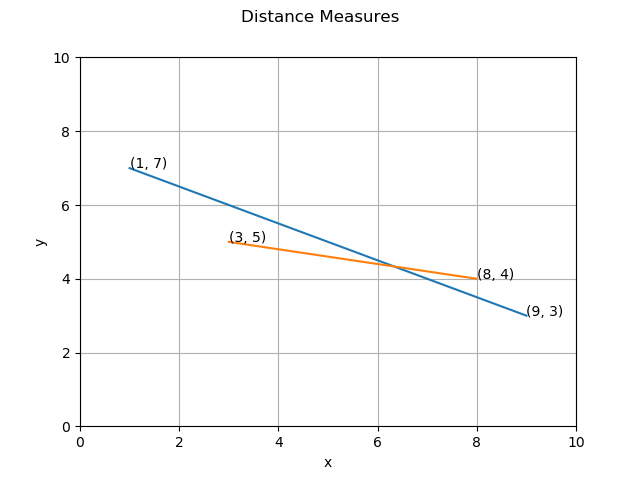
\includegraphics[width=.7\textwidth]{image/general/distance.png}
\caption{Example of Distance Measure}
\label{fig:distanceMeasure}
\end{figure}

To further accentuate on the concept of distance measure in this work, a simple example of how distance metrics can be applied in the proposed method is illustrated using Figure \ref{fig:distanceMeasure} with two plotted lines. In order to simplify the research problem, these lines can be thought of as vehicle trajectories captured over time that is flatten unto a 2D plot. Using the available data, the distance between two trajectories can be measured and used to signify the dissimilarity between them. This distance measure can also be used to identify trajectories with high resemblance. 

\begin{figure}[hbt!]\centering
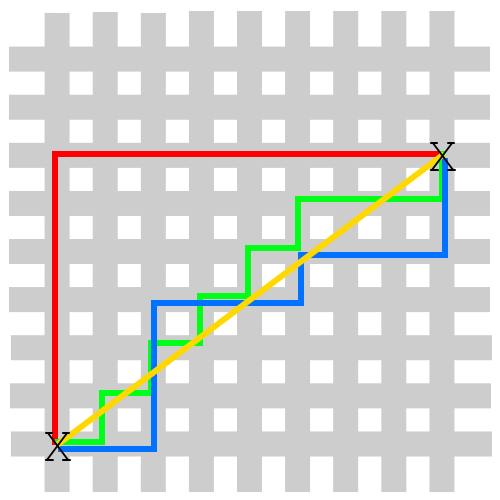
\includegraphics[width=.5\textwidth]{image/lit/manhattan.png}
\caption[Comparison between Manhattan Distance vs. Euclidean Distance]{With the assumption that each block has a equal distance of 1. Using Manhattan Distance, regardless of the path taken, the distance for the red, green and blue lines has the length of $14$. These 3 paths, while different, still takes on the shortest distance from one end to the other. However, when computing using Euclidean Distance, the distance is measured to be $\sqrt{8^2+6^2} = 10$. Euclidean Distance only produces $1$ unique solution while Manhattan Distance may produce more than one solution.}
\label{fig:manhattan}
\end{figure}


However, as different distance measure metrics are suitable for different scenarios, a good distance measure is an essential for comparing a significantly extensive set of vehicle trajectories during the retrieval process of a car park scene. This concept of distance measure was further extended into a multi-dimensional space such as the colours space, where the similarity between two or more colours were measured using different distance metrics to evaluate the performance of each metric. Table \ref{table:distance} lists out several distance measure which are commonly used along with the pros and cons of each while Figure \ref{fig:manhattan} shows the contrast between Euclidean and Manhattan distance.

\begin{table}[!ht]
\resizebox{\textwidth}{!}{
\begin{tabular}{|l|l|l|}
\hline
\textbf{Distance Measure} & \textbf{Pros} & \textbf{Cons} \\ \hline
Euclidean Distance & \begin{tabular}[c]{@{}l@{}}Simple, Fast,\\ Commonly used,\\ Able to work on n-Dimension data\end{tabular} & \begin{tabular}[c]{@{}l@{}}Vector order dependent,\\ Requires same length vectors\end{tabular} \\ \hline
Manhattan Distance & \begin{tabular}[c]{@{}l@{}}Reflection invariant,\\ Translation invariant,\\ Produces same result,\\ Able to work on n-Dimension data\end{tabular} & \begin{tabular}[c]{@{}l@{}}Requires same length vectors,\\ Does not have a unique solution\end{tabular} \\ \hline
Chamfer Distance & \begin{tabular}[c]{@{}l@{}}Able to work with \\ vectors of different length,\\ Vector order invariant, \\ Minimizes the difference \\ between vectors,\\ Able to work on n-Dimension data\end{tabular} & \begin{tabular}[c]{@{}l@{}}Higher computational cost,\\ Alternative matches may \\ receive equal distance\end{tabular} \\ \hline
Hamming Distance & \begin{tabular}[c]{@{}l@{}}Ensure similarity between vectors,\\ Able to work on n-Dimension data\end{tabular} & \begin{tabular}[c]{@{}l@{}}Vector order dependent,\\ Requires same length vectors\end{tabular} \\ \hline
\end{tabular}%
}
\caption{List of several distance measures along with their pros and cons}
\label{table:distance}
\end{table}




\subsection{Human Visual System}
\label{section:eyes}
The human eyes are visual system organs, responsible of receiving and processing visual information. Figure \ref{fig:eyes} shows a rough anatomy of the human eye. Within the eye, rods and cones are light-sensitive cells, found on the retina which are in charge of vision. Both of these cells plays a different role, rods cells are not able to perceive colour information, hence, they are known to be responsible for determining the lighting condition. On the other hand, cones cells are responsible for the reception of colour information. As human retina contains approximately 120 million rods and 6 million cones, the eyes are more sensitive toward lighting conditions. The sheer number of rods also enables humans to see in low-light achromatic vision.   


\begin{figure}[hbt!]\centering
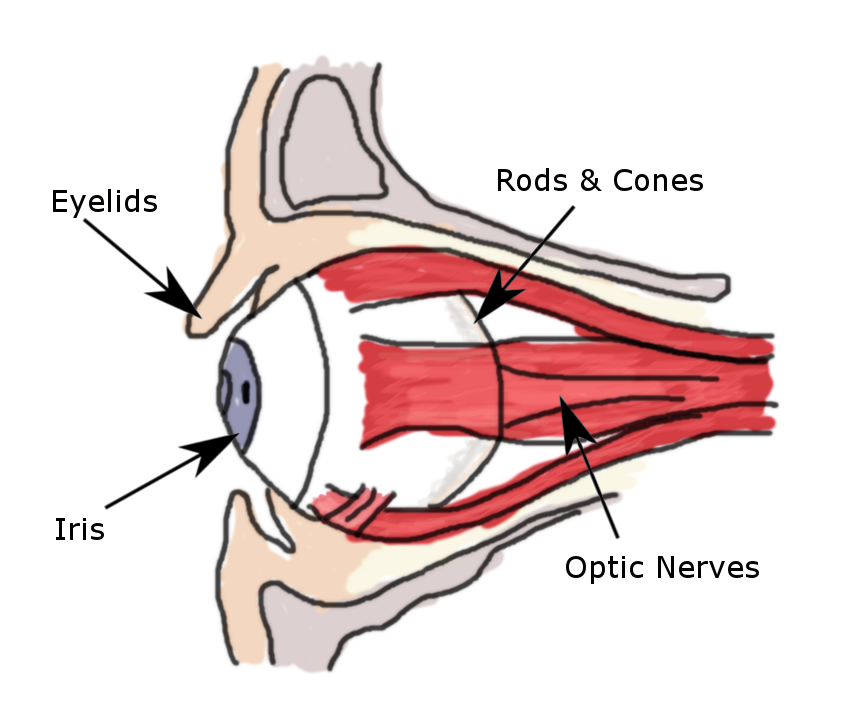
\includegraphics[width=.5\textwidth]{image/lit/rodsandconscolored.png}
\caption[Human Eye Anatomy]{Human Eye Anatomy. Rods and cones cells are responsible over human vision. When these cells on the retina are stimulated, signals are sent to the brain via the optic nerves. The brain would then processes these signals to provide vision for humans.}
\label{fig:eyes}
\end{figure}

Anatomically, there are three types of cones in the human retina, each of which are responsible over the receptiveness of colours in a particular type of wavelength. These wavelengths can be classified into three main categories: Short wavelengths light, Medium  wavelengths light and Long wavelengths light (See Figure \ref{fig:visibleSpectrum} \cite{eyespectrum}). colours are perceived from the combination of stimuli to these rods and cones cells and responses from brain. When stimulated, these cells fires electrical signals to the optic nerves fibres that communicates with the brain. However, as the number of cones cells in the retina varies for each person, the colour perception of everyone would differ in a way or another. 


\begin{figure}[hbt!]\centering
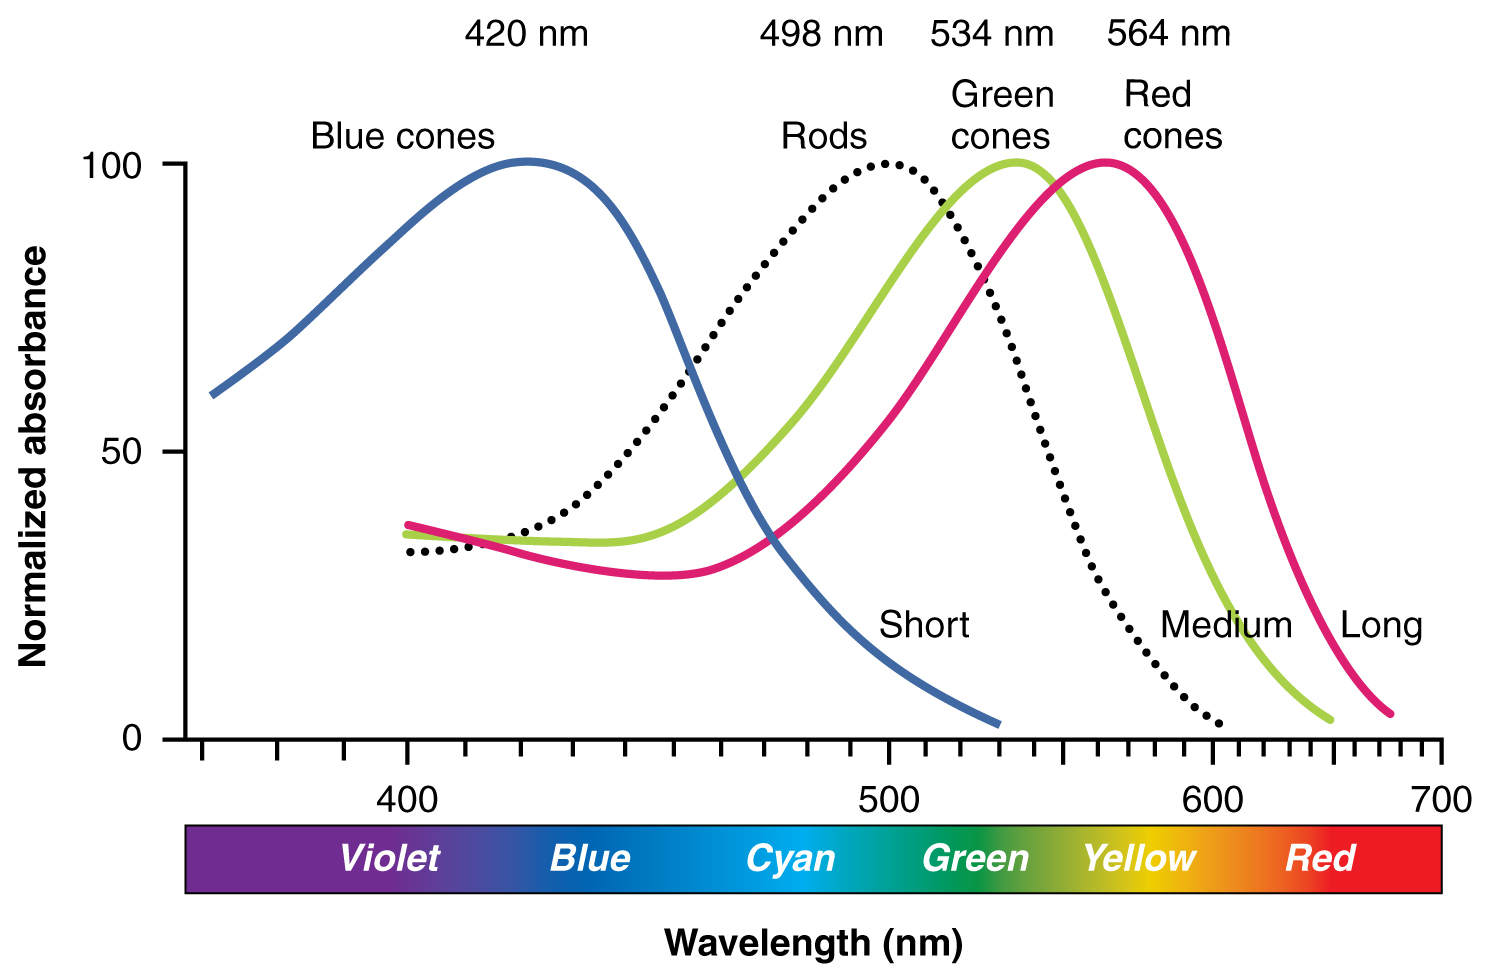
\includegraphics[width=.7\textwidth]{image/lit/ColorSensitivity.jpg}
\caption[Normalised human photo-receptor absorbency rate for different wavelength lights]{Normalised human photo-receptor (cons \& rods) absorbency rate for different wavelengths of light. 'Blue' cones, approximately 420-440 nm, are short wavelengths light; 'Green' cones, approximately 534-545 nm, are medium wavelengths light; and, 'Red' cones, approximately 564-580 nm, are long wavelength lights }
\label{fig:visibleSpectrum}
\end{figure}




\subsection{Colour Model, Systems and Terms}
\label{section:colourterm}

In order to represent colours in tuples of number, colour models were designed. In essence, it can be thought of a quantization process of converting a series of real-world continuous signal (colour wavelengths) into a set of finite tuples of numbers within a colour model. 
With the ability to quantize these wavelengths into sets of finite tuples, the colours can be digitised and used for further processing.


\subsubsection{Colour Models}
From the previous section, the humans' visual system was explored. From there, it is learnt that the cones cells in the retina are strongly receptive towards stimuli of 'Red', 'Green' and 'Blue' wavelengths. Given the solid theory behind human perception of colours, the RGB colour model was designed. This colour model is commonly used to represent and display images in digital systems. 

As an example, the RGB colour space is an additive colour model, each of the components (R, G, B) are added together to produce the final colour. Typically each of these components are represented using 8 bits, hence, 256 possibilities for each component with a total of $256 \times 256 \times 256 = 16M$ colour combinations in total. As this is an additive model, 'Black' colour is  represented using $(0, 0, 0)$, while 'White' using $(255, 255, 255)$. Figure \ref{fig:rgb} represents this colour model.

\begin{figure}[hbt!]\centering
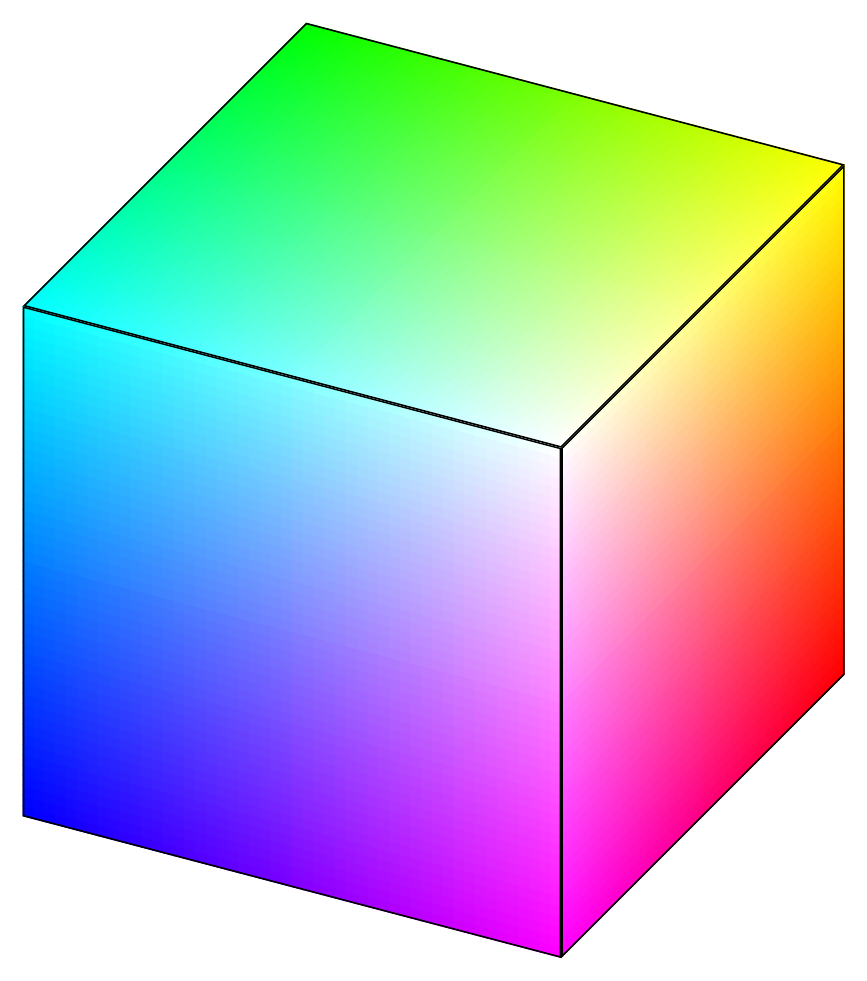
\includegraphics[width=.4\textwidth]{image/lit/rgbcolor.jpg}
\caption{RGB colour Model}
\label{fig:rgb}
\end{figure}


\subsubsection{Munsell Colour System}
\label{section:munsellcs}
colour terms - such as "Red", "Green" or "Blue", are commonly derived from the Munsell colour system which was created in the early 20th century by Professor Albert H. Munsell. The Munsell colour System was designed to organise colours similar to how the human's eye sees - which is, by organising colours according to their hues, followed by the chromatic range and the brightness values in a perceptually uniform manner. 

For each horizontal circle on the Munsell colour System, the hues can be divided into 5 principle hues which are Red, Yellow, Green, Blue, and Purple. This setup allows another 5 intermediate hues in between each principle hues, for example: Green-Blue hue, Purple-Red hue. 
Figure \ref{fig:munsell}(a) illustrates the Munsell colour System while Figure \ref{fig:munsell}(b) illustrates the property of the chroma and value scale available on the Munsell colour system, for example, a hue at 2.5 Yellow-Red (YR) has a maximum chroma value which differs along the value axis. 



\begin{figure}[!htb]
  \centering
  \resizebox{\textwidth}{!}{
\begin{tabular}{cc}
 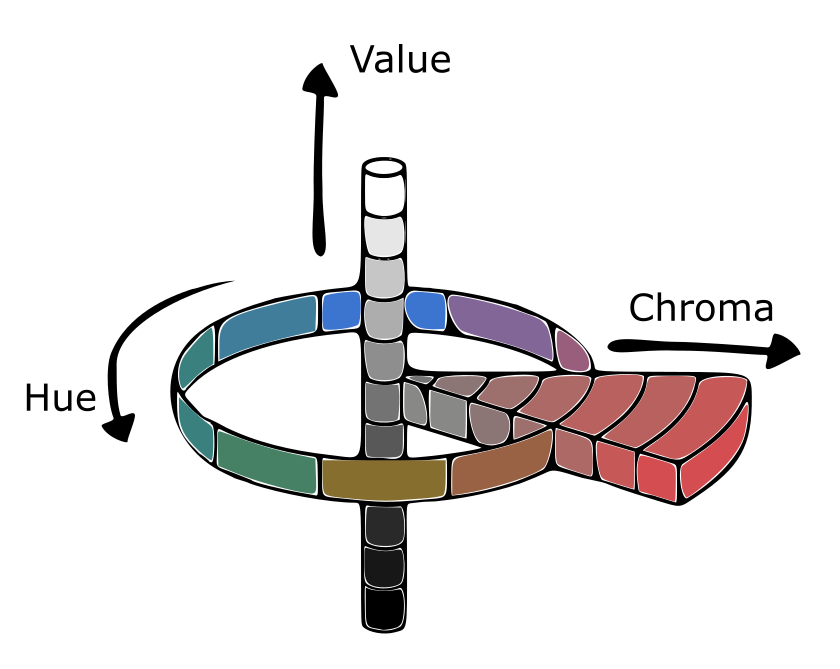
\includegraphics[width=0.4\linewidth]{image/general/munsell.png}  &
 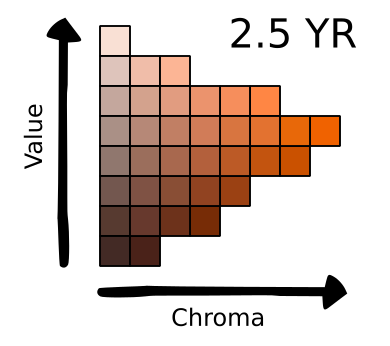
\includegraphics[width=0.4\linewidth]{image/general/25YR.png}\\
 (a) Munsell colour System &
(b) Hue at 2.5YR with various Chroma and Value\\
\end{tabular}}
\caption{Munsell colour System} \label{fig:munsell}
\end{figure}



\subsubsection{Colour Terms}

While the basic idea of colours seems to be a relatively simple idea for humans, machines on the other hand, do not understand the concept of colours. Modern computers generally represents colour values using the Red-Green-Blue (RGB) values for most applications. Despite its frequent usage, it is difficult for humans to visualise a particular colour when presented with three RGB values as these values does not directly translate the intuitive nature of a particular colour. Along with that, it is also very difficult to visualise the difference between two colours using the RGB values only. 

Table \ref{table:allcolourterms} lists several popular web colour dictionaries along with the number of colour terms as well as the publishing year. One notable property of these colour terms is the use of compound terms such as 'baby blue', 'dark red', 'light purple' and 'very deep brown'. Along with that, in some colour dictionary, certain colours terms are duplicated for several tuples. Given the variety of colour dictionaries and the number of different colour terms, one of the targets in this work is to investigate and decide how many colour terms should be allocated to describe the vehicle colours. 

\begin{table}[hbt!]
\centering
\begin{tabular}{|c|c|c|}
\hline
\multicolumn{1}{|c|}{\textbf{Web Colour Dictionary}} & \multicolumn{1}{c|}{\textbf{Number of Colour Terms}} & \multicolumn{1}{c|}{\textbf{Year}} \\ \hline
x11 (R3)                                            & 631                                                 & 1988                               \\ \hline
HTML                                                & 140                                                 & Current                            \\ \hline
CSS                                                 & 148                                                 & Current                            \\ \hline
Crayola                                             & 248                                                 & Current                            \\ \hline
xkcd                                                & 954                                                 & 2010                               \\ \hline
\end{tabular}
\caption[Web Colour Dictionary and the corresponding number of colour terms]{Web Colour Dictionary and the corresponding number of colour terms}
\label{table:allcolourterms}
\end{table}

%https://people.csail.mit.edu/jaffer/colour/Dictionaries
% x11 colours: https://groups.google.com/forum/?fromgroups=#!topic/comp.windows.x/AYPozZhQxok
% https://www.crayola.com/explore-colours.aspx
%http://markkness.net/colourpy/colourPy.html



In a classic study of worldwide colour naming, \citeA{berlinandkay} proposed that the naming of colours terms may differ due to different cultures. Based on their findings, native English language speakers generally used eleven basic colour terms. These terms had to have three common properties which are: i) Highly used, ii) Monolexemic - meaning a single(mono) word, and not compounded colour term such as 'baby blue', and iii) agreed upon by native speakers of the language. With those definitions, the common colour terms proposed for the English language are black, white, gray, brown, red, orange, yellow, purple, green, blue, and pink. The 11 common colour terms were also adopted by several other authors (\citeA{van2009learning}, \citeA{zaslavsky2018efficient}, and \citeA{yu2018beyond}) in their work to understand how these colour terms can be used for real-world image applications. However, \citeA{yu2018beyond} also remarked that most existing work on colour names focuses on only the eleven basic colour terms of the English language, however, this could be limiting the discriminative power of these representations. 







\section{Related Works}
\label{section:relatedworks}

The advancement of computer vision technologies enabled the development and integration of various solutions to tackle challenges in Intelligent Transportation Systems (ITS). As ITS is a big topic, there has been a substantial increase of research done on the various subdomains. With the amount of research done, instead of reinventing the wheel, existing frameworks were adopted and leveraged upon. Recent survey done by \citeA{tian2017hierarchical} and \citeA{chandran2017review} were studied to understand the general overview of the state of related works. The authors has summarised the challenges that are often found in an ITS setting that is implemented on a one-camera setup: 
\begin{enumerate}
    \item \textbf{Camera placement} affects the overall performance. 
    \item The \textbf{lighting condition} varies throughout the day. Supplemental lighting equipment can be used during the night, however, the visual range will be limited.
    \item Vehicles are often \textbf{occluded} in an ITS setting; often by pedestrians, bicycles, trees, and even buildings.
    \item \textbf{Vehicle pose} varies when turning or changing lanes.
    \item Vehicles comes in a \textbf{variety of shapes, sizes, and colour.}
    \item As \textbf{vehicles' size changes} as it pass through the camera's field of view. This variation in visual information affects the robustness of some detection models. 
\end{enumerate}
Along with that, \citeA{tian2017hierarchical} presented an overview of the general frameworks for ITSs with the aim of vehicle attribute extraction and behaviour understanding in Figure \ref{fig:ITSoverview}. According to \citeA{liu2016deep}, in a real-world scenario, appearance features such as colours, shapes, and types are very effective to filter out the dissimilar vehicles. In addition, they are efficient to be extracted and searched in large-scale dataset. 
As mentioned in Section \ref{subsec:scope}, the bounding box of each vehicles are assumed to be obtained prior to the semantic extraction task, related literature regarding the detection and tracking of vehicles will not be discussed. 
Instead, the rest of this section is expounded under two main categories: i) Objects Semantic Extraction, and ii) Object Semantic Retrieval. 


\begin{figure}[hbt!]\centering
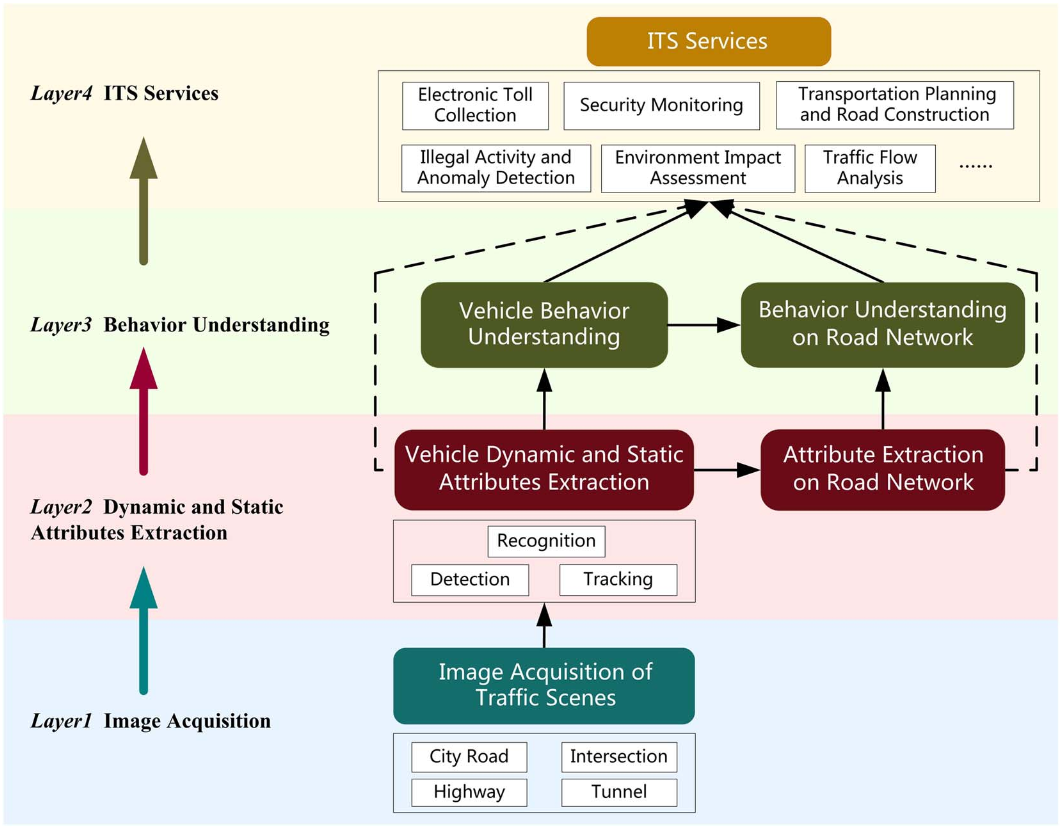
\includegraphics[width=1\textwidth]{image/lit/ITS.png}
\caption[Overview of the General Frameworks for ITSs]{(From Bottom) Layer 1: The process of obtaining data via vision sensors. Layer 2: Attribute Extraction from data; this includes motion, trajectories, colours, shapes and etc. Layer 3: Analysis on vehicle behaviours from the extracted attributes to decide traffic status. Layer 4: Utilises information from Layer 3 to optimise various ITS services. Figure reproduced from~\citeA{tian2017hierarchical}}
\label{fig:ITSoverview}
\end{figure}




\subsection{Object Semantics Extraction}

\subsubsection{Vehicle Colours Extraction}
The extraction of Vehicle colours is essential for a wide variety of applications in ITS such as crime prevention and security purposes. 
According to \citeA{zhang2017vehicle}, colour is one of the most stable attributes of vehicles and often used as a valuable cue in some important applications.
\citeA{hsieh2015vehicle}, \citeA{chen2014vehicle} and \citeA{zhang2017vehicle} noted that in a surveillance scenario, the varying illumination, coupled with complex environment factors (weather, noise) as well as the camera viewpoint in an outdoor scene affected the classification of colours drastically. 
Various vehicle colour extraction methods has been proposed in the recent years, these methods can be broadly divided into two main categories: i) Hand Crafted Features, and ii) Machine Learned Features.
In \citeA{hsieh2015vehicle}'s work, the vehicles are grouped into seven categories (Figure \ref{fig:sevenclasses}). Given that the source footages were taken outdoor with varying illumination settings, a global colour correction method (Figure \ref{fig:colorcorrection}) was employed to suit different lighting needs. 

\begin{figure}[hbt!]\centering
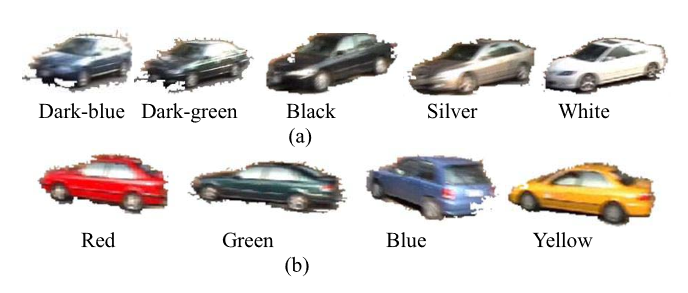
\includegraphics[width=.8\textwidth]{image/lit/carscolors.png}
\caption[Colour Appearance Categories of  Vehicle  Used  for  Colour Classification]{(a) Vehicles Classified as "Achromatic"; (b) Chromatic Vehicles. Reproduced from \citeA{hsieh2015vehicle}.}
\label{fig:sevenclasses}
\end{figure}

\begin{figure}[!htb]
  \centering
 \resizebox{\textwidth}{!}{
\begin{tabular}{ccc}
 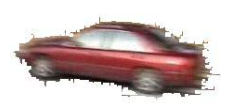
\includegraphics[width=0.4\linewidth]{image/lit/windowremove1.png}  &
 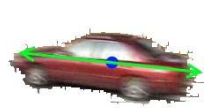
\includegraphics[width=0.4\linewidth]{image/lit/windowremove2.png} & 
 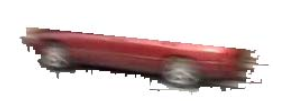
\includegraphics[width=0.4\linewidth]{image/lit/windowremove3.png} \\
 (a) Input Vehicle &
(b) Proposed Cutting Line for Window Removal &
(c) Result of Window Removal\\
\end{tabular}
}
\caption[Window Removal Task. From left: Input Vehicle, Proposed Cutting Line, Results of Window Removal]{Window Removal Task. From left: Input Vehicle, Proposed Cutting Line, Results of Window Removal. Image reproduced from \citeA{hsieh2015vehicle} \label{fig:windowremoval}}
\end{figure}

\begin{figure}[!htb]
  \centering
  \resizebox{\textwidth}{!}{
\begin{tabular}{cccc}
 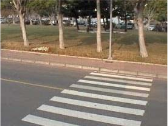
\includegraphics[width=0.3\linewidth]{image/lit/cc1.png}  &
 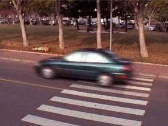
\includegraphics[width=0.3\linewidth]{image/lit/cc2.png} & 
 
\includegraphics[width=0.3\linewidth]{image/lit/cc4.png} & 
 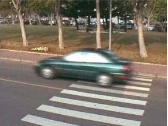
\includegraphics[width=0.3\linewidth]{image/lit/cc3.png} \\
 (a) Reference Image &
(b) Colour Distortion &
(c) Background of (b) &
(d) Result of Colour Correction\\
\end{tabular}
}
\caption[Colour Correction. From left: Reference Image, Image with Colour Distortion, Background of (b), Results of Colour Correction]{Colour Correction. From left: Reference Image, Image with Colour Distortion, Background of (b), Results of Colour Correction. Image reproduced from \citeA{hsieh2015vehicle} \label{fig:colorcorrection}}
\end{figure}

Along with that, occasionally the vehicle windows appear white due to the effects of specular highlights, the authors also proposed a window-removal task to increase the accuracy (Figure \ref{fig:windowremoval}). This work also proposed the classification of vehicles into chromatic and achromatic classes, the final colour category is decided via Support Vector Machine (SVM). The accuracy of differentiating between chromatic and achromatic classes over 10,000 vehicles were reported to be approximately 88\%. \citeA{chen2014vehicle} also suggested a similar approach by implicitly selecting a Region-of-Interest (ROI) to improve the classification performance for both images and video data. These collected data were captured using high-definition cameras with resolutions of $1920 \times 1080$ pixels. In this work, the ROI in the image was selected by assigning different weights which are learnt by a classifier for each of the proposed subregions. 

\citeA{jeong2017homogeneity} took on a different approach in order to extract the vehicle colours by implementing a Homogeneity Patch Search Method. In their work, a voting system as implemented to vote on the dominant colour based on the HSV histograms which were extracted from each patch using Adaboost Classifier. First, the edges from the input image was detected using Sobel edge operators. Next, Distance Transformation was performed using Felzen-szwlb algorithm to obtain the minimal distance to the edges of each pixel. As edges often introduce distortion of colour, this step allows the proposed method to select patches that further from the edges. Figure \ref{fig:colorpatches} illustrates this process. While \citeA{jeong2017homogeneity}'s proposed method obtained an accuracy of 92\% over 7 classes, it was only tested against 208 images that have a relatively high resolution of $1624 \times 1224$ pixels.

\begin{figure}[!htb]
  \centering
  %\resizebox{\textwidth}{!}{
\begin{tabular}{cc}
 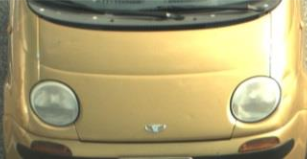
\includegraphics[width=0.3\linewidth]{image/lit/homo1.png}  &
 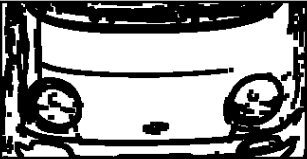
\includegraphics[width=0.3\linewidth]{image/lit/homo3.png} \\
(a) ROI Image &
(b) Inverse of Edge Image \\
 
\includegraphics[width=0.3\linewidth]{image/lit/homo2.png} & 
 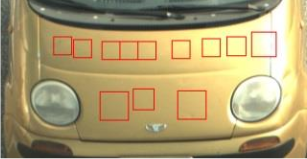
\includegraphics[width=0.3\linewidth]{image/lit/homo4.png} \\
(c) Distance Transformation &
(d) Selected Patches\\
\end{tabular}
%}
\caption[Homogeneity Patch Search from Input. (a) Region of Interest, (b) Inverse of Edge Image Using Sobel Operators, (c) Distance Transformation Calculated using Felzen-szwlb algorithm, (d) Selected Patches Based on Obtained Distance.]{Homogeneity Patch Search from Input. (a) Region of Interest, (b) Inverse of Edge Image Using Sobel Operators, (c) Distance Transformation Calculated using Felzen-szwlb algorithm, (d) Selected Patches Based on Obtained Distance. Image reproduced from \citeA{jeong2017homogeneity} \label{fig:colorpatches}}
\end{figure}

As colour histograms are one of the most common feature used for colour classification task, \citeA{kim2008deciding} aimed to understand the correlation of the number of colour histogram bins used and how different configurations would affect the performance of matching the histogram bins to colour terms using distance measures. This use of histogram bins effectively reduces the processing time needed while promoting recognition accuracy \cite{zhang2017vehicle}. The Hue-Saturation-Intensity (HSI) colour space was used with a total of 17 varying configurations of histogram bins (e.g. 16 bins for Hues, 4 bins for Saturation and 4 bins for Intensity) for the experiment. The results from the experiment shows an average score of 84\%; the best configuration of (H:8, S:4, I:4) achieved an accuracy of 87.83\% over seven colour classes with 100 images per class. 

\citeA{zhang2017vehicle} and \citeA{hu2015vehicle} approached this challenge of extracting colour term by implementing a convolutional neural network (CNN) to extract deep features which are then fed into a linear SVM for the classification task. \citeA{zhang2017vehicle} mentioned that the state-of-the-arts methods takes the whole image for colour recognition, however many parts of the images such as car windows, wheels, and background contributes negatively to the recognition accuracy. A noise reduction method via saliency detection was proposed in order to boost the performance. While this method achieved an accuracy of 94\%, the proposed pipeline with saliency detection, deep feature extraction, dual-orientational dimensionality reduction and classifier training is not suitable for real-time applications.

\begin{figure}[!htb]
  \centering
  %\resizebox{\textwidth}{!}{
\begin{tabular}{cc}
 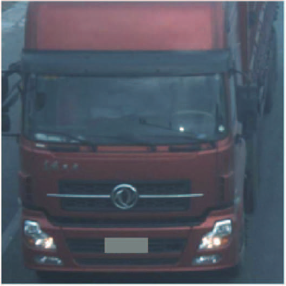
\includegraphics[width=0.4\linewidth]{image/lit/hu1.png}  &
 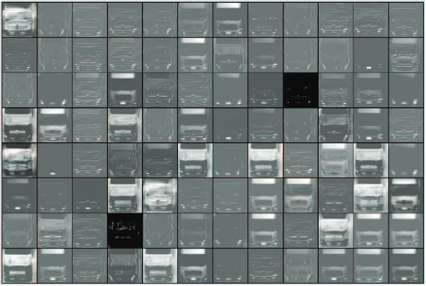
\includegraphics[width=0.6\linewidth]{image/lit/hu2.png} \\
(a) Input Image &
(b) Response Map of the First Convolutional Layer \\
\end{tabular}
%}
\caption[(a) Input and (b) Response from First Convolutional Layer. ]{(a) Input and (b) Response from First Convolutional Layer. Image reproduced from \citeA{hu2015vehicle} \label{fig:responseFCL}}
\end{figure}

According to \citeA{hu2015vehicle}, there are two reason of choosing SVM over fully-connected layers (FCL). The first reason is the ability of SVMs to perform better due to the regularisation contraints that helps overcome overfitting of training data. Another reason why SVM was chosen was due to the fact that SVMs has lesser parameters, this makes the fine tuning process easier. 
Figure \ref{fig:responseFCL} illustrates the input image and the response produced by the first convolutional layer produced in \citeA{hu2015vehicle}'s work. The author claims that the proposed method has advantages over hand-crafted methods that performs the segmentation of subregions, this is because the response map from the first convolutional layer contains meaningful ROIs which are effective for distinguishing vehicle colours. This work achieved an average precision of 93\%, with input data of $1920 \times 1080$ resolution.  
As a whole, while both hand crafted features and machine learnt features methods were able to achieve an accuracy of over 84\%, most of the proposed solutions worked on high resolution data.   

\begin{figure}[hbt!]\centering
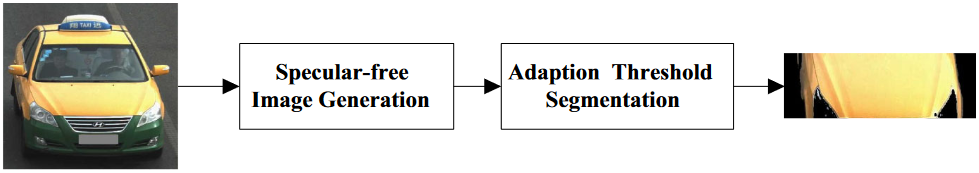
\includegraphics[width=1\textwidth]{image/lit/salient1.png}
\caption[Vehicle-Colour Saliency Detection]{Vehicle-Colour Saliency Detection. Reproduced from \citeA{zhang2017vehicle}.}
\label{fig:Colorsaliency}
\end{figure}

In a semi-related research area of vehicle re-identification, several authors ( \citeA{liu2016deep}, \citeA{liu2016deep2} and \citeA{shen2017learning}) made use of extracted colour features to assist with the re-identification process. \citeA{liu2016deep} adopted the Probabilistic Latent Semantic Analysis (PLSA) introduced by \citeA{van2009learning} to extract the colour features. A PLSA model is used to learn the relation between words (colour terms) and images by providing a conditional probability score. Similar to the work of \citeA{kim2008deciding}, the images in this work were segmented and represented using L*a*b colour histogram of $10 \times 20 \times 20$ grids. \citeA{liu2016deep2} applied deep learning techniques inspired by a triplet loss network proposed by \citeA{ding2015deep}, the network used a new loss function to accelerate the training convergence. The colour features were extracted using the proposed network. Similarly, \citeA{shen2017learning} applied a deep learning network to extract the colour features using a Siamese Network with a shared ResNet-50 configuration. The visual features, including colours, were obtained using the features from the global pooling layers.

\subsubsection{Colour to Colour Term Mapping}

Colour terms are very useful in a real-world application instead of colour tuples. According to \cite{van2009learning}, colour names are required for image retrieval and image annotation applications. 
Several authors has looked into mapping colour tuples into their respective colour terms. \citeA{van2009learning} proposed several variants of Probabilistic Latent Semantic Analysis (PLSA) model to learn colour names from data obtained Google Images. 
This was done in order to avoid hand-labelling real-world images with colour names, Figure \ref{fig:van20091} illustrates the types of images retrieved using Google Images. The authors approach this challenge by comparing their methods against 3 chip-based methods. 
In their work, chip-based methods was described as colour naming method that is performed in a controlled environment where the labels of colour chips are placed on a neutral background under a known white light source. 
Similar to \citeA{van2009learning}'s work, \citeA{yu2018beyond} also applied PLSA to estimate the probability of colour values when given a colour term.

\begin{figure}[hbt!]\centering
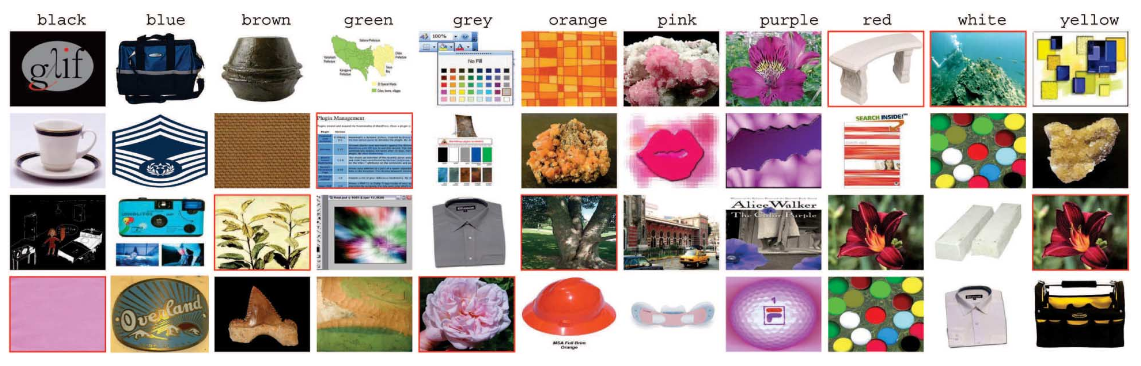
\includegraphics[width=1\textwidth]{image/lit/van20091.PNG}
\caption[Google-retrieved examples for colour names. The red bounding boxes indicate false positives. An image can be retrieved with various colour names, such as the flower image which appears in the red and the yellow set.]{Google-retrieved examples for colour names. The red bounding boxes indicate false positives. An image can be retrieved with various colour names, such as the flower image which appears in the red and the yellow set.  Reproduced from \citeA{van2009learning}.}
\label{fig:van20091}
\end{figure}

The PLSA model allows multiple colour terms to be named for each image. The pixels in the image (document) was discretized (quantized) into a finite vocabulary set of $10 \times 20 \times 20$ cubes of L*a*b colour space. Then, the image was represented using a histogram which indicates how many pixels are assigned to each bin (word). Now, given a set of documents $D = \{d_1, d_2, ... , d_N\}$ each described in a vocabulary $W = \{w_1, w_2, ... , w_M\}$, the words are taken to be generated by latent topics $Z = \{z_1, z_2, ... , z_K\}$. In the PLSA model the conditional probability of a word $w$ in a document $d$ is given by:
\begin{align}
    p(w|d) = \sum_{z\in Z}{p(w|z)p(z|d)}
\end{align}
The aim of $p(w|d)$ is to find latent topics which best explains the observed data, and in this case, finding the colour terms that best describes an image. In their approach, the authors claim that it their proposed method is flexible when new colour terms are introduced to any given system as the model can be trained with a small amount of data as compared to traditional methods which relies on chip based studies. 

In the works of \citeA{khan2013discriminative} and \citeA{yu2018beyond}, the authors suggests that colour representation that has been extended to more than the eleven dimensions could be beneficial. The authors in \cite{yu2018beyond} proposed a dataset of 28 additional colour terms (a total of 39 terms) which was used in their experiments on several task such as visual tracking, person re-identification as well as image classification. One of their experiments shows that the classification accuracy has improved by 4\% when changing from 11 to 25 colour terms. 



\begin{figure}[hbt!]\centering
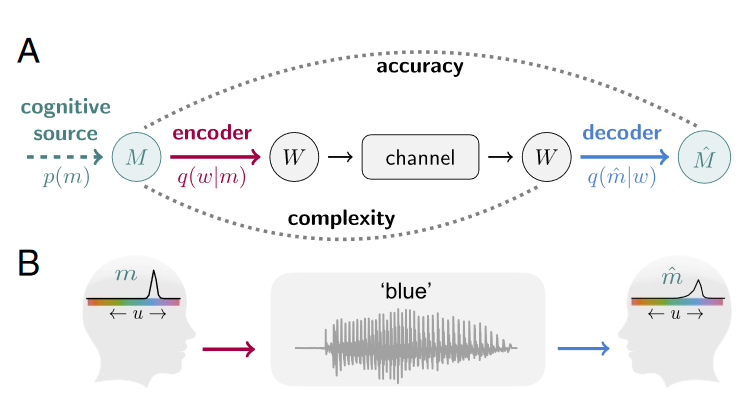
\includegraphics[width=1\textwidth]{image/lit/datacompress1.PNG}
\caption[(A) Shannon's communication model. In this model, the source message $M$ and its reconstruction $\hat{M}$ are distributions over objects in the universe $U$. We refer to these messages as meanings. $M$ is compressed into a code, or word, W. We assume that $W$ is transmitted over an idealised noiseless channel and that the reconstruction $\hat{M}$ of the source message is based on $W$. The accuracy of communication is determined by comparing $M$ and $\hat{M}$, and the complexity of the lexicon is determined by the mapping from $M$ to $W$. 
(B) Colour Communication Example,  where $U$ is a set of colours, shown for simplicity along a single dimension. A specific meaning $m$ is drawn from $p(m)$. The speaker communicates $m$ by uttering the word “blue”, and the listener interprets blue as meaning $\hat{m}$.
]
{(A) \citeA{shannon1948mathematical}'s communication model. In this model, the source message $M$ and its reconstruction $\hat{M}$ are distributions over objects in the universe $U$. We refer to these messages as meanings. $M$ is compressed into a code, or word, W. We assume that $W$ is transmitted over an idealised noiseless channel and that the reconstruction $\hat{M}$ of the source message is based on $W$. The accuracy of communication is determined by comparing $M$ and $\hat{M}$, and the complexity of the lexicon is determined by the mapping from $M$ to $W$. 
(B) Colour Communication Example,  where $U$ is a set of colours, shown for simplicity along a single dimension. A specific meaning $m$ is drawn from $p(m)$. The speaker communicates $m$ by uttering the word “blue”, and the listener interprets blue as meaning $\hat{m}$.
Reproduced from \citeA{zaslavsky2018efficient}.}
\label{fig:datacompression1}
\end{figure}

The work of \cite{zaslavsky2018efficient} took on another approach towards colour tuples mapping. The authors aimed to study efficient compression in colour naming and its evolution. \citeA{zaslavsky2018efficient} claims that colour categories cannot be hard-partitioned in the colour space, instead, a soft-partitioned approach should be taken. However, with a soft-partition approach, there are transition regions in the colour space that are often inconsistently named. 
In their work, the approached this challenge of understanding how colours are named from the angle of data compression. Figure \ref{fig:datacompression1} illustrates the idea of \citeA{zaslavsky2018efficient}'s work. The goal of this work is to design a Information Bottleneck (IB) compression model that represents can effectively represent colours terms in different languages. 








\begin{comment}
https://ieeexplore.ieee.org/stamp/stamp.jsp?tp=&arnumber=4982667&tag=1
https://www.pnas.org/content/pnas/115/31/7937.full.pdf
https://link.springer.com/content/pdf/10.1007%2Fs00138-017-0902-y.pdf
https://www.imbs.uci.edu/~kjameson/HinksCardenasKuehniEtAlJOSA2007.pdf
http://imbs.uci.edu/~kjameson/ECST/Kay_Cook_WorldColorSurvey.pdf
http://www.munsellcolourscienceforpainters.com/ConversionsBetweenMunsellAndsRGBsystems.pdf


\end{comment}




\subsubsection{Vehicle Motion Extraction \& Representation}
\label{subsec:vehiclemotionextraction}

Vehicle motion is an important feature that can be used to describe activities in a car park surveillance scene. While there are not many research done within the scope of a car park surveillance setting, there has been many works in the ITS domain which extracts vehicle motions. In most cases where the research setup involves a static camera sensor, the extraction of these motions can be broadly divided into two groups: i) Background subtraction (BGS) methods combined with vehicle centroid position for motion estimation; and ii) Extraction of features (Eg: Scale-Invariant Feature Transform (SIFT), Histogram of Oriented Gradients (HOG), Haar-like, Kanade-Lucas-Tomasi (KLT)) which are combined with Optical flow for motion estimation. 
However, as described in Section \ref{subsec:scope}, the bounding box of the vehicles is assumed to be provided.
Hence, a brief overview of the vehicle motion extraction process will be explored while trajectory representation methods are discussed in detail. 


BGS methods are often used as there is no need of prior training on a machine to recognise vehicles, instead this method relies on captured motions.
Several authors (\citeA{wang2016research, luvizon2017video, apeltauer2015automatic}) extracted vehicle motion information via BGS method. Generally, a clean model of background information is first obtained. When a new object is introduced on the scene in the current frame, the differences between the background information and the current frame is extracted to indicate changes in the scene. When the objects (blobs) are moving in the scene, the data obtained from the subtraction process would correspond to motion information. Figure \ref{fig:bgs2} illustrates the process involve in BGS. In order to further increase the accuracy, these works filters out blobs that does not match the desired dimensions. 

\begin{figure}[hbt!]\centering
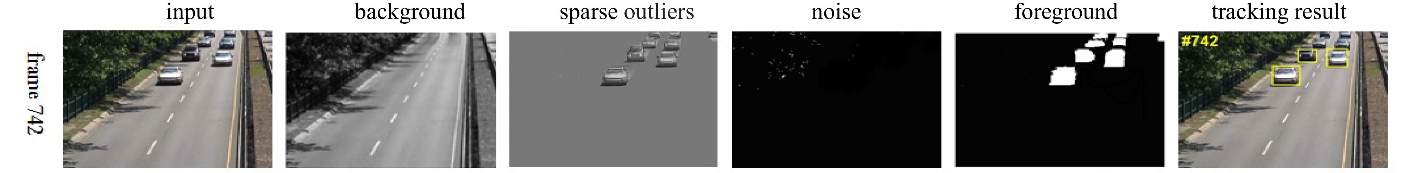
\includegraphics[width=1\textwidth]{image/lit/bgs.PNG}
\caption[Vehicle Motion Extraction using Background Subtraction. From left: Input, Background Model, Sparse Outlier, Noise, Foreground, Tracking Result]
{Vehicle Motion Extraction using Background Subtraction. From left: Input, Background Model, Sparse Outlier, Noise, Foreground, Tracking Result.
Reproduced from \citeA{yang2017real}.}
\label{fig:bgs2}
\end{figure}

Contrary to BGS methods, feature extraction methods relies on visual information of vehicles such as colours, texture and shapes. In the case of vehicles, the combination different components such as the windscreen, doors, wheels and windows adds up to be a vehicle. These visual information are learned to model and identify vehicles.
Several authors \cc{fill up who used features like these}
In the attempt of counting vehicles from 500 hours of videos, \citeA{lessard2016countingapp} applied the works of \citeA{saunier2006feature} to extract motion information using KLT tracker. Next, these extracted features were grouped into unique trajectories that varies depending on the targeted scene. In their work, some scenes were allocated up to 12 different types of unique trajectories. Using this method, the authors was able to uniquely identify the different types of motion, however, this method is not feasible when dealing with  datasets in the wild as there are too many variables and parameters to account for. Furthermore, the process of annotating the data would be too laborious. 

Instead of manually allocating unique trajectories, \citeA{momin2015vehicle} took a different approach of categorising motions. The authors combined haar-like features along with BGS methods to extract motion information. The extracted vehicle motions at each point in time is then split into one of the four directions (LEFT, RIGHT, UP, DOWN). Similarly, the works of \citeA{feris2012large} splits the motion of vehicles into 12 motion directions depending on the orientation of the vehicles. These motion directions were assigned for every $\ang{30}$ (eg: $\ang{0}-\ang{30}, \ang{30}-\ang{60}, \cdots, \ang{330}-\ang{360}$). A motion direction histogram was built such that bins which receives the highest number votes were assigned as the motion direction saved into the database. Likewise, \citeA{castanon2016retrieval} categorised motions into 9 histogram of motion bins using the aggregate motion which was computed using pixel-level optical flow (Horn and Schunck method). These 9 bins corresponds to the eight cardinal directions along with one idle bin to denote the absence of significant motion.


With the goal of designing huge repositories of moving vehicle trajectories, \citeA{d2015designing} represent trajectories using spatio temporal cubes (See Figure \ref{fig:spatiocube}). 
Similarly, \citeA{lai2015video} represented trajectories of human's trajectories in this manner. In addition to that, the authors used B-spline curve fitting methods to further reduce noisy information. As different degrees of curve fitting leads to different results (see Figure \ref{fig:spatiocube2}), the authors proposed to merge multiple curves of different degrees to strike a balance between noise removal and accuracy.
This method of trajectory representation using spatio temporal cubes is intuitive as it is able to capture and relay information accurately. 
However, the downside of this method is that the accuracy of data representation heavily relies on the number of spatio-temporal cubes used. 

\begin{figure}[hbt!]\centering
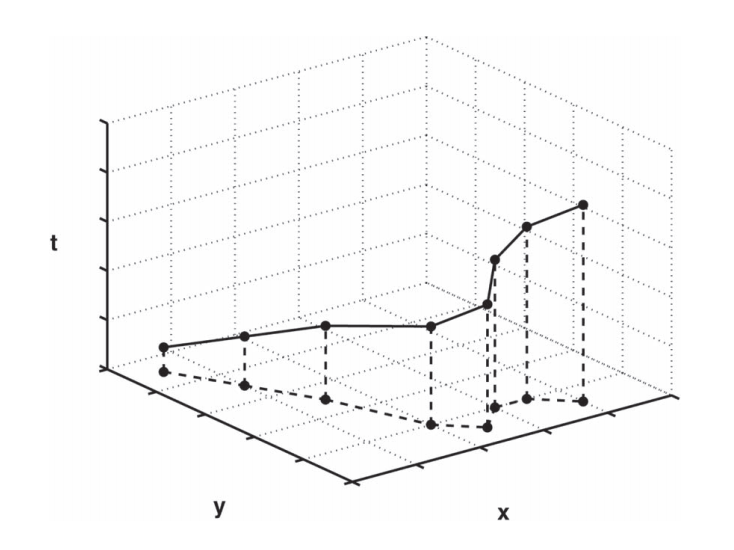
\includegraphics[width=.5\textwidth]{image/lit/spatiotemporal.PNG}
\caption[Representation of Trajectories in a Spatio-temporal Cube.]
{Representation of Trajectories in a Spatio-temporal Cube.
Reproduced from \citeA{d2015designing}.}
\label{fig:spatiocube}
\end{figure}

\begin{figure}[hbt!]\centering
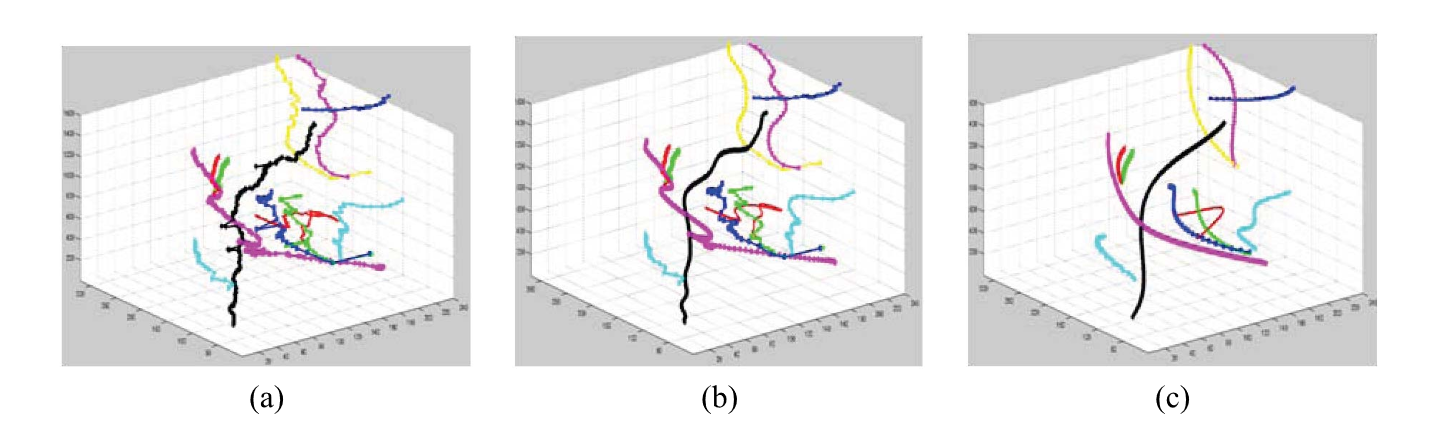
\includegraphics[width=1\textwidth]{image/lit/spatiotemporal2.PNG}
\caption[Representation of Human Trajectories in a Spatio-temporal Cube. (a) Original Object Trajectories; (b) Curve fitting results using high degrees; (c) Curve fitting results using low degrees.]
{Representation of Human Trajectories in a Spatio-temporal Cube. (a) Original Object Trajectories; (b) Curve fitting results using high degrees; (c) Curve fitting results using low degrees.
Reproduced from \citeA{lai2015video}.}
\label{fig:spatiocube2}
\end{figure}



\subsection{Object Semantics Retrieval}

According to the survey by \cite{chandran2017review}, object retrieval algorithms can be broadly divided into two categories: i) String Matching Algorithm, and ii) Sketch Matching Algorithm. String matching algorithms typically converts subjects into a set of known keywords and match them using its semantic meanings. However, \citeA{bhaumik2016hybrid} suggests that Content-based Video Retrieval (CVBR) can be classified into three categories: i) Classical Approach, ii) Soft Computing and iii) Hybrid Soft Computing. Figure \ref{fig:cvbr} presents a classification of the various approaches used in CVBR systems.

\begin{figure}[hbt!]\centering
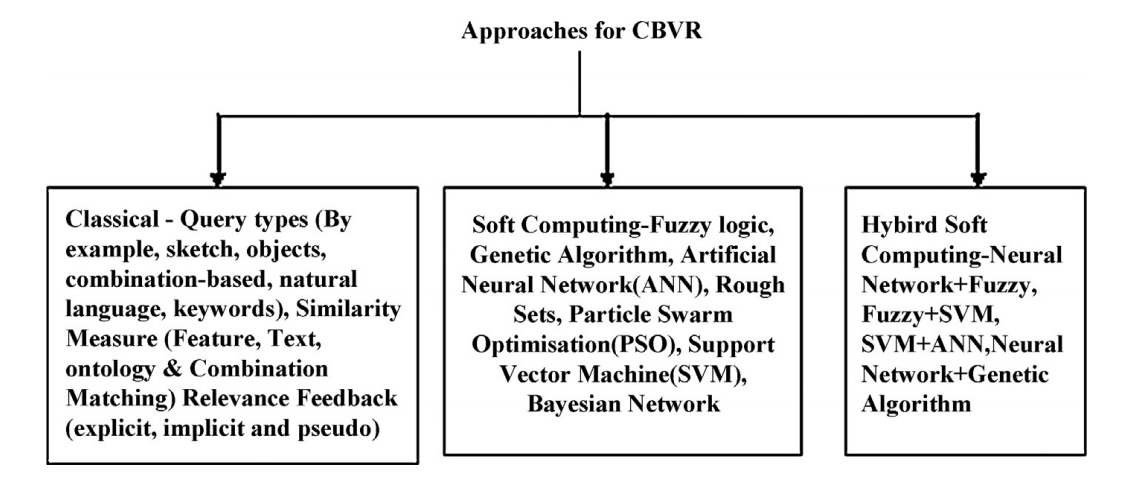
\includegraphics[width=.7\textwidth]{image/lit/cvbr.PNG}
\caption[Classification of Approaches Used in Content-based Video Retrieval Systems.]
{Classification of Approaches Used in Content-based Video Retrieval Systems.
Reproduced from \citeA{bhaumik2016hybrid}.}
\label{fig:cvbr}
\end{figure}

Several authors (\citeA{feris2012large}, \cite{momin2015vehicle}, and \cite{yang2015semantic}) has implemented string matching algorithms (classical approach) in their work. In the case of vehicle trajectories, often the queries are represented in the form of keywords such as "Turning into junction A" or "Enter from entrance B". The approach suggested by these authors attempts to simulate natural language queries that would be provided by end users. However, when dealing with large datasets that contains a variety of scenes, it is difficult to adopt this approach as it is not feasible to manually assign keywords. In a review, \citeA{bhaumik2016hybrid} claims that the use of textual queries has been proven to be ineffective in video retrieval systems. This is because keywords may not be able to capture the type of semantic content required by a end user.

Within the exemplar-based retrieval, the use of sketch approach is another classical method applied by retrieval engines.
\citeA{flickner1995qbic} proposed a retrieval engine which takes in queries in the form of features such as object motion, colours, shapes and texture. Similarly, \citeA{Cheng_2013_ICCV} also took on the challenge of retrieving contents based on the detected salient regions. However, the author only focused on the retrieval of still images instead of videos. In terms of retrieval of trajectories, \citeA{lai2015video} allowed end users to draw trajectories that matches the desired results. These drawn trajectories will then be fitted using B-spline curves which will then be use to match against the records stored in the database. The authors reported an average accuracy of 73.28\% when tested against 5 video sequence with an average length of 1500 frames. Figure \ref{fig:drawquery1} illustrates the hand drawn trajectories which are converted into query inputs.


\begin{figure}[hbt!]\centering
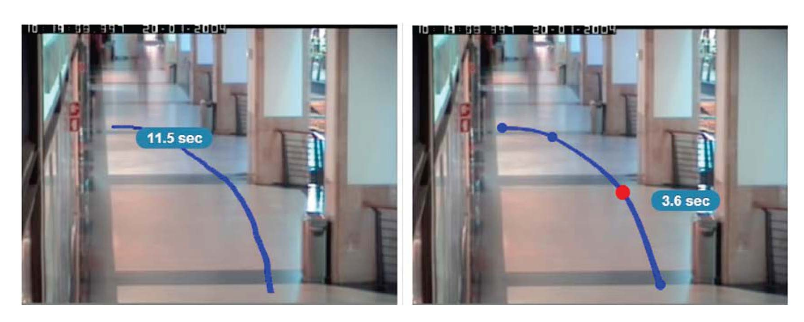
\includegraphics[width=.9\textwidth]{image/lit/trajdraw1.PNG}
\caption[\textit{Left}: Hand-drawn Trajectory for Retrieval Purposes. \textit{Right}: Resulting Simplified B-spline Curve for Easier Manipulation of Trajectory. ]
{\textit{Left}: Hand-drawn Trajectory for Retrieval Purposes. \textit{Right}: Resulting Simplified B-spline Curve for Easier Manipulation of Trajectory.
Reproduced from \citeA{lai2015video}.}
\label{fig:drawquery1}
\end{figure}

Similar to the approach taken by \cite{lai2015video}, in an airborne video setting, \citeA{castanon2016retrieval} also allowed end users to draw the trajectories which are then segmented and used for the retrieval purposes. The authors applied dynamic programming techniques to search for the best match. Along with that, the authors also reported that their approach takes an average of 2.9 seconds to process one frame for a simpler task while taking up to 4.32 seconds to process a single frame in a complicated task. The processing speed was averaged out across 2000 frames. This approach appears to be rather computationally expensive. However, the authors reports significantly better results when compared to other methods.Figure \ref{fig:drawquery2} illustrates the proposed GUI and the input queries while Figure \ref{fig:rocresult} reports the performance of the proposed method.


\begin{figure}[hbt!]\centering
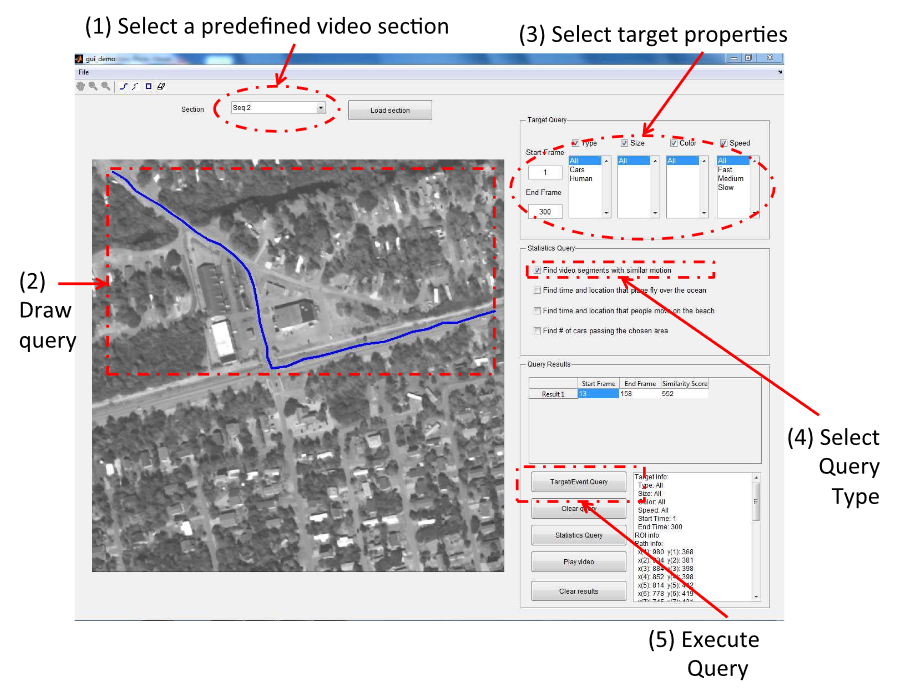
\includegraphics[width=.6\textwidth]{image/lit/trajdraw2.PNG}
\caption[Graphical User Interface and the Input Trajectory.]
{Graphical User Interface and the Input Trajectory.
Reproduced from \citeA{castanon2016retrieval}.}
\label{fig:drawquery2}
\end{figure}

\begin{figure}[hbt!]\centering
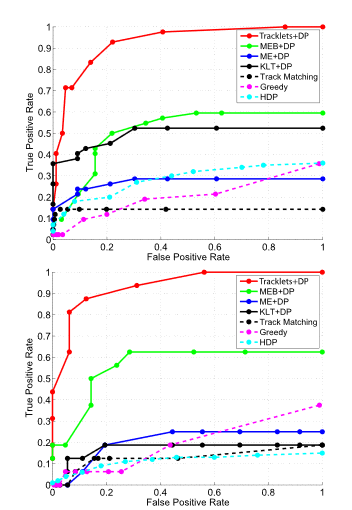
\includegraphics[width=.6\textwidth]{image/lit/roc.PNG}
\caption[ROC Curve for Cars and Human Trajectories in Airborne Data.]
{ROC Curve for Cars and Human Trajectories in Airborne Data
Reproduced from \citeA{castanon2016retrieval}.}
\label{fig:rocresult}
\end{figure}

%!TEX ROOT = thesis.tex
\chapter{Framework Overview}

\section{Introduction}
In order to tackle the issues discussed in the earlier through the literature review as well as the various motivations, the theoretical framework is laid as to provide a conceptual schema on how to break the rather huge and intricate challenge into multiple bite sized puzzles. This chapter is organized as such, first, the overview of the framework used in this work is described in Section \ref{section:framework}, followed by some reoccurring key concepts throughout this work in Section \ref{section:keyconcepts}. Next, the description of the dataset used is described in Section \ref{section:dataset_used} and finally, this chapter concludes with the experimental methodology applied in this work (see Section \ref{sec:expmethodology}). 


\section{Framework Overview}
\label{section:framework}
In this section, a high level overview of the fundamental processing step along with two suggested core components for vehicle semantic extraction and retrieval is provided. The groundwork described in this work abides to the typical top-down approach used in Intelligent Transportation System (ITS) where the video data is subjected to background subtraction, followed by blob filtering, vehicle detection as well as vehicle tracking is as described in \cite{lim2017}. 

The semantic information from the vehicle blobs are then extracted and stored in the database. With the vehicle specific semantics stored in the database, retrieval engines were designed to enabled users to easily retrieve the stored information. Both retrieval engines features a graphical user interface which allowed users to enter the queries by drawing the desired trajectory as well as entering other crucial information which would assist in identifying the targeted video shot.


\begin{figure}[hbt!]\centering
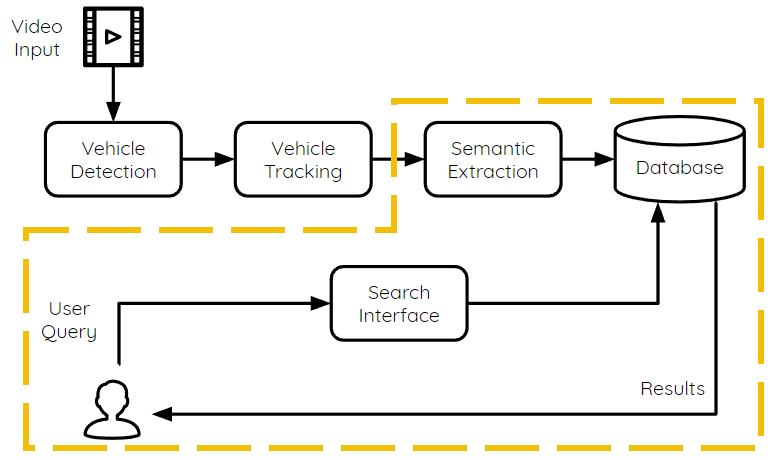
\includegraphics[width=.9\textwidth]{image/framework_new.PNG}
\caption{Framework Diagram, Contribution in Highlighted Border}
\label{fig:framework}
\end{figure}


In this work, two frameworks were suggested and used for the vehicle semantic extraction and retrieval process. Both of which utilizes an underlying distinctive approach, with the same end goal in mind, which is the retrieval of desired video snippets which closely resembles a user described query. For each of these frameworks, the formulation of idea, steps and process involved are described in this chapter. As there are various solutions proposed in this work, solutions which are common to both core frameworks is also provided. As a whole, the end-to-end framework can be visualized using Figure \ref{fig:framework} where the main contribution of this work is highlighted in yellow border. 

\subsection{LSH-Inspired Retrieval Framework}
The first of the two frameworks suggested in this work is the \textit{LSH-Inspired Retrieval Framework}. Locality-Sensitve Hashing (LSH) refers to a technique used for dimensionality reduction, typically to perform hashing on a set of documents so that documents with similar properties are mapped and clustered to similar locality or neighbourhood. This technique excels especially when working with high dimensional data such as video data in this work.

By building on top of the fundamental processing step, the semantics from each vehicle blobs are extracted

\subsection{Chamfer Distance based Framework}




\section{Key Concepts}
\label{section:keyconcepts}
In this section, a reoccurring key concept used in the proposed method is discussed as to provide a high level understanding. 

\cc{try to expound more on this part}


\subsection{Quantization}

The use of quantization in the mathematical and digital signal processing field is no longer a new concept. However, digital signal processors are limited by natural boundaries such as hardware limitations, and are only able to compute and perform arithmetic operations within a limited range \cite{spors_2018}. The use of quantization refers to the process of mapping and projecting a set of large values which are often continuous or analog in nature into a set of discrete and finite values. 

\begin{figure}[hbt!]\centering
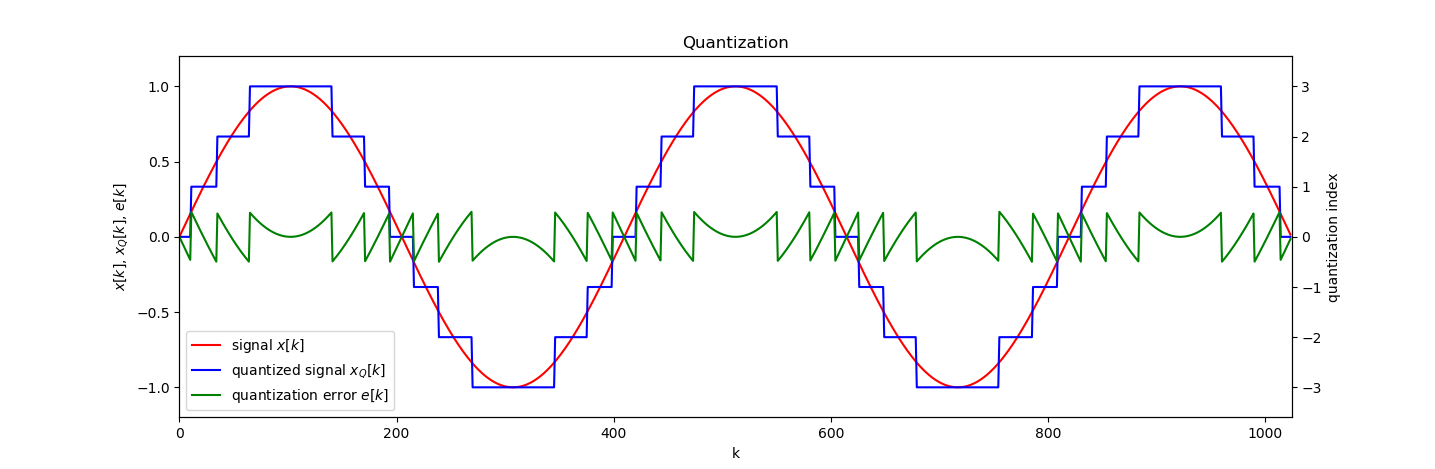
\includegraphics[width=\textwidth]{image/general/quantization.png}
\caption{Quantization}
\label{fig:framework}
\end{figure}


The use of quantization enables reduction in memory usage (compression) as well as to reduce computational cost which leads to faster processing speed. However, since quantization is a many-to-few mapping operation, hence, the operation is considered irreversible without prior knowledge of the loss. Nevertheless, the output discrete signal can closely resemble the input continuous signal depending on the number of quantization index used.   

In the proposed method, the quantization technique was extended further into a three dimensional space where the 3D space is quantized into a set of discrete and finite values to ease the calculation and manipulation of data in the both the video data as well as the color space. 

\begin{equation}\centering
\label{eq:quantization}
x_Q[k] = g( \mspace{3mu}\lfloor \mspace{3mu}f(x[k]) \mspace{3mu}\rfloor\mspace{3mu})
\end{equation} 

\vspace{-3em}


\begin{equation}\centering
\label{eq:quantizationerror}
e[k] = x_Q[k] - x[k]
\end{equation}


In order to expound on the quantization process, a mathematical model of this process can be formulated as such. Consider a continuous signal $x[k]$ whose quantized signal, $x_Q[k]$, is desired. The functions $f (\mspace{3mu} \cdot  \mspace{3mu})$ \& $g (\mspace{3mu} \cdot  \mspace{3mu})$ can be thought of as a real-value mapping function while the $\lfloor \mspace{3mu} \cdot  \mspace{3mu} \rfloor$ represents a rounding function. As previously mention, this process is considered irreversible with prior knowledge of the loss, in this case, the quantization error, $e[k]$, can be computed using the Equation \ref{eq:quantizationerror}. 

\subsection{Distance Measure}

The use of distance metrics is another reoccurring key concept in the proposed method. While distance measure is commonly used in computer science as well as the mathematics field, there are numerous metrics suggested by different authors which are applicable and useful in different scenarios.   

In the proposed method, the use of distance metrics allows the author to measure the performance of the proposed algorithms. A simple example of how distance metrics is applied in the proposed method can be illustrated using Figure \ref{fig:distanceMeasure} where the distance between two lines signifies the dissimilarity between them. 



\begin{figure}[hbt!]\centering
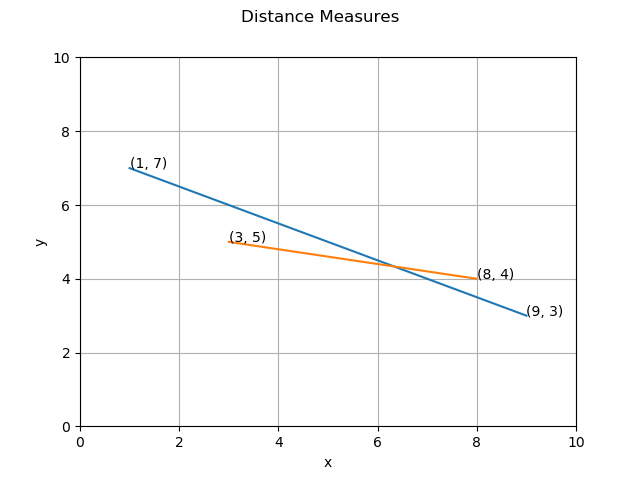
\includegraphics[width=.7\textwidth]{image/general/distance.png}
\caption{Example of Distance Measure}
\label{fig:distanceMeasure}
\end{figure}

As different distance measure metrics are favourable in different scenarios, a good distance measure when used in a carpark scene is essential when comparing a significantly extensive set of vehicle trajectories during the retrieval process.   

Again, this concept was further extended into a multi-dimensional space such as the colors space, where the similarity between two or more colors was measured using different distance metrics to evaluate the performance of each metric. 



\subsection{Color Model}

While humans' visible spectrum $(400nm - 700nm)$ can be represented using the respective wavelengths,  in order to describe these values in a 

\cc{to fill up... talk about color space and why}
%http://markkness.net/colorpy/ColorPy.html

\begin{figure}[hbt!]\centering
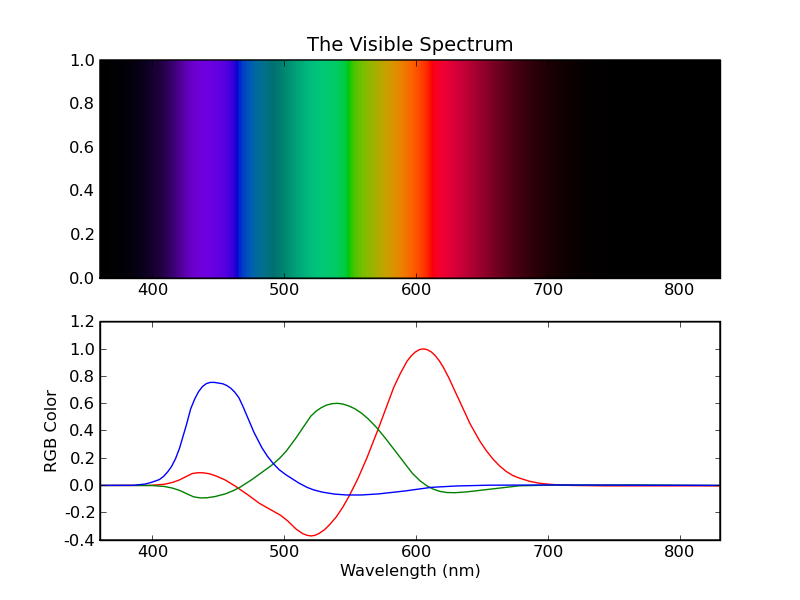
\includegraphics[width=.7\textwidth]{image/general/VisibleSpectrum.png}
\caption{RGB Values and their corresponding spectrum}
\label{fig:distanceMeasure}
\end{figure}





\section{Dataset}
\label{section:dataset_used}

In view of testing the proposed framework for large-scale extraction and retrieval of video semantics, a new collection of video dataset was gathered. A stationary cloud-enabled web camera was set up on the fourth floor of a building with a window facing a piece of private carpark area. Figure \ref{fig:camerasetup} depicts the camera setup overcasting the carpark area. 

The aforementioned setup was done to mimic a typical camera setup which tower over a piece of outdoor carpark lot that are found in the wild. 


\begin{figure}[hbt!]\centering
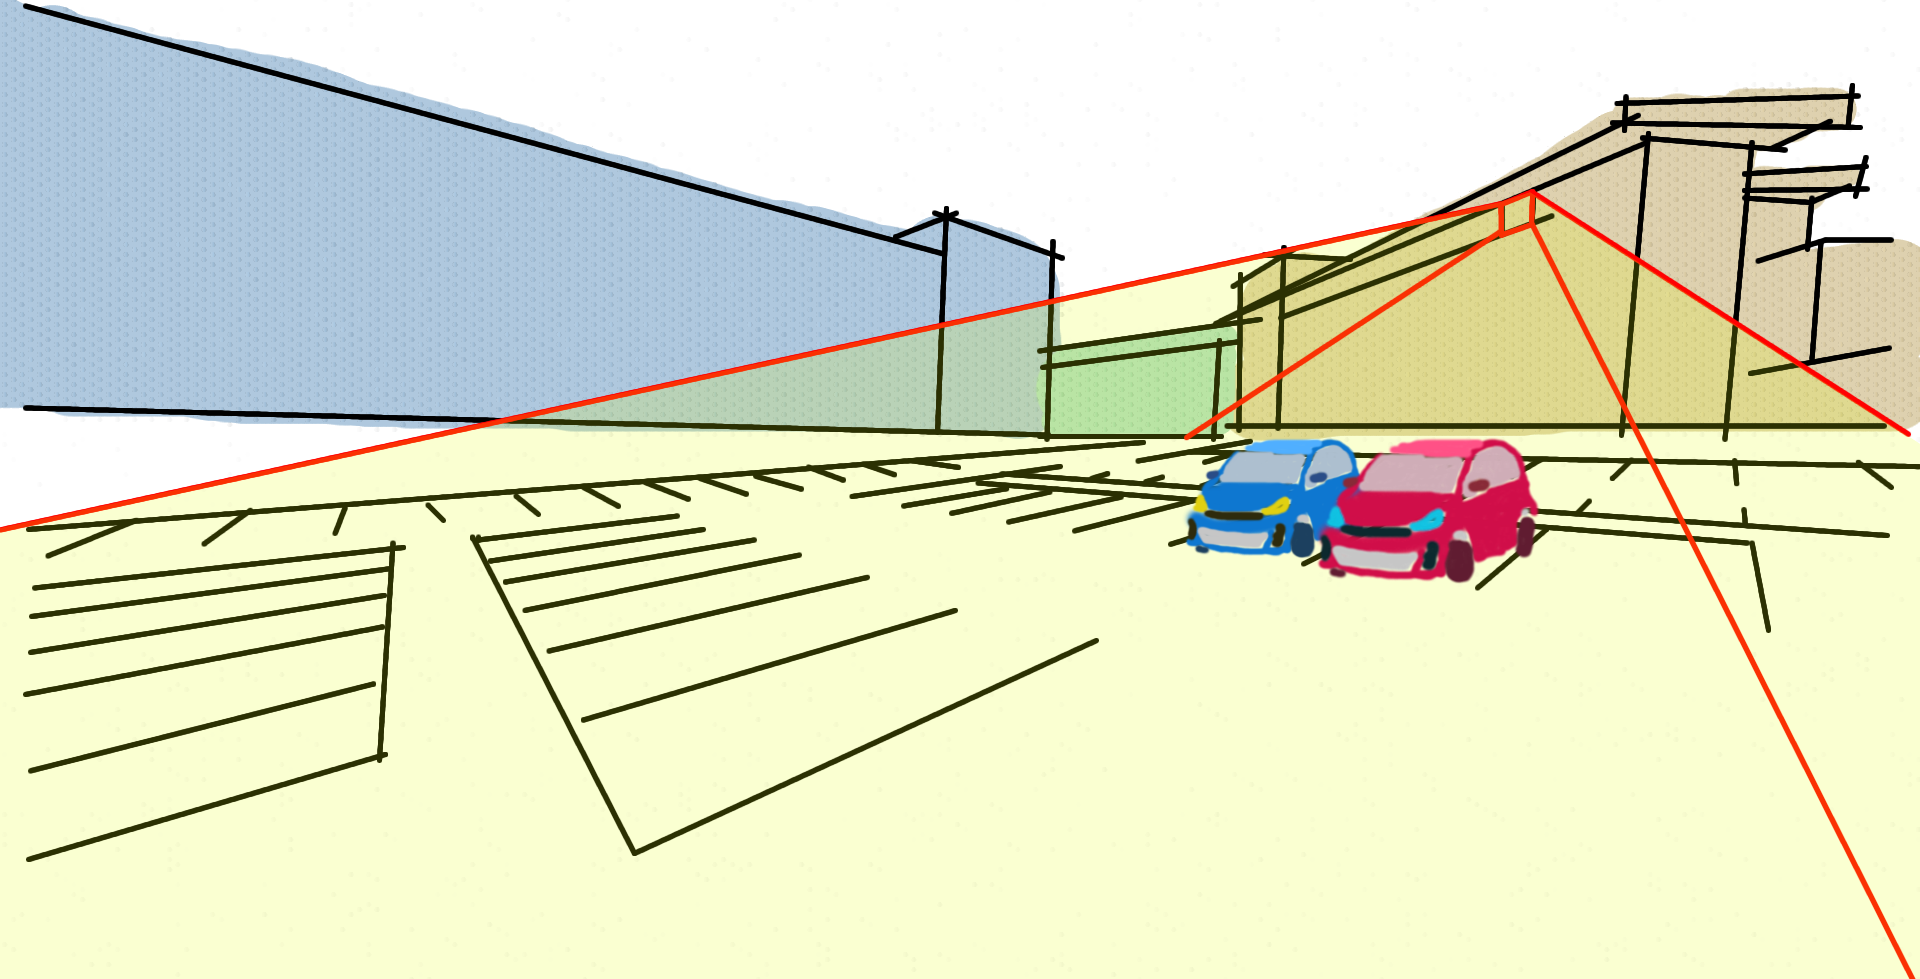
\includegraphics[width=.8\textwidth]{image/fcicarpark2.png}
\caption{Camera setup to capture the carpark from the fourth floor}
\label{fig:camerasetup}
\end{figure}


\begin{figure}[hbt!]\centering
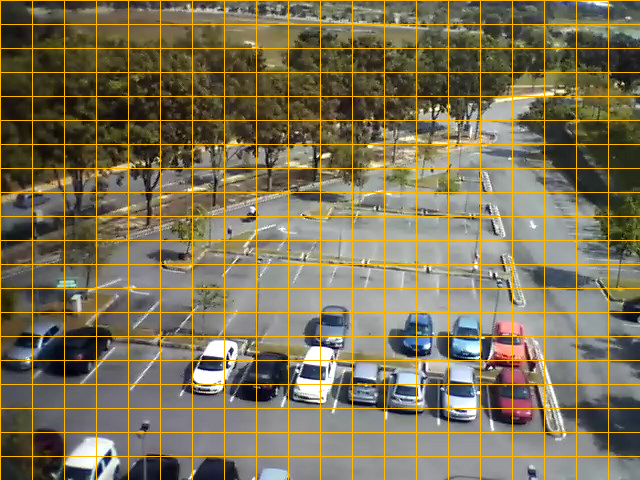
\includegraphics[width=.7\textwidth]{image/general/grids.png}
\caption{View from camera setup; 20$\times$20 Grids}
\label{fig:viewfromcamera}
\end{figure}


Through the camera's web interface, this device was set to record on weekdays from Monday through Friday, starting from 08:30 in the morning up until 18:30 in the evening, with a total of 10 hours was recorded each day. Among the important settings, each recorded video clip was set to have a maximum length of 6 minutes, and hence, 10 video clips every hour, and a total of 100 at the end of each day. The recorded video clips were saved into the external microSD memory card. At the end of each day, the data was then copied over to a server via a script. However, due to glitches that occurred during the recording process, some of the video clips were cut off abruptly. Hence, some of the days do not contain the full 10 hours video clips. 

\begin{table}[]\centering
\begin{tabular}{ll}
Camera Model: & Dlink DSC-942L        \\
Resolution:   & 640$\times$480 pixels \\
Frame rate:   & 10 $fps$             \\
Format:       & H.264 / MPEG-4 AVC    \\
Naming Convention: & $CCYYMMDD\_HHMMSS.mp4$
\end{tabular}
\vspace{1em}
\caption{Camera details}
\end{table}

\begin{figure}[htb!]
  \centering

\begin{tabular}{cc}
 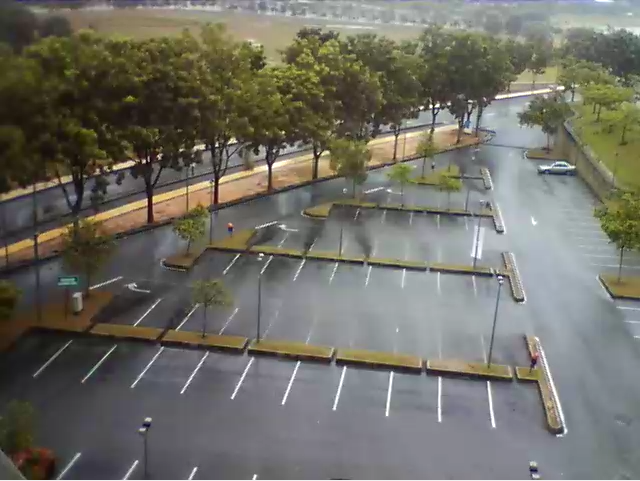
\includegraphics[width=0.4\linewidth]{image/general/rain.PNG} &  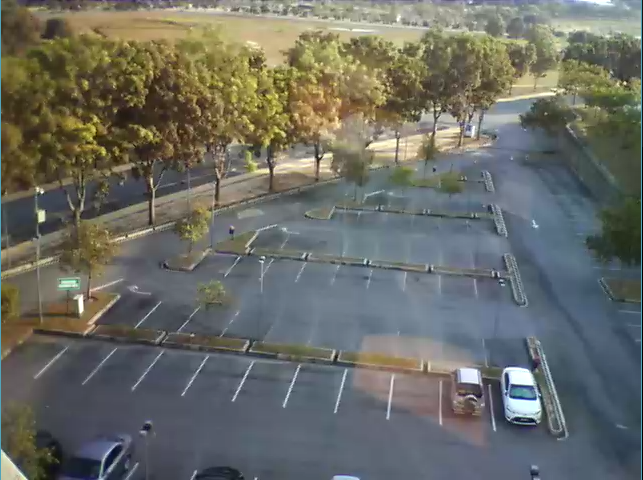
\includegraphics[width=0.4\linewidth]{image/general/reflection.PNG}\\ 
\begin{tabular}{c}(a) Rainy day with \\ reflective surface\end{tabular} & \begin{tabular}{c}(b) Reflection on the \\carpark from the window\end{tabular} \\
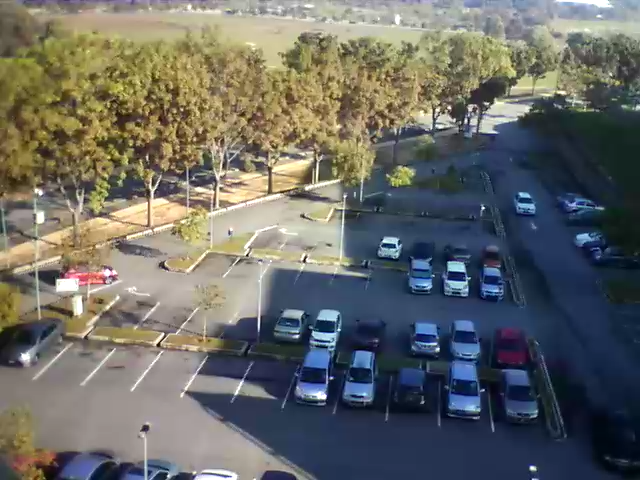
\includegraphics[width=0.4\linewidth]{image/general/shadow.png} &  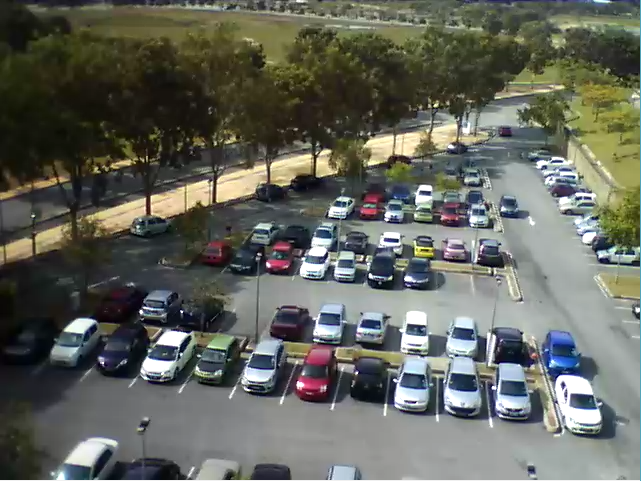
\includegraphics[width=0.4\linewidth]{image/general/shadow2.png}\\
\begin{tabular}{c}(c) Severe shadow over \\ the car park (08:48AM)\end{tabular} & \begin{tabular}{c}(d)  Severe shadow over \\ the car park (04:06PM)\end{tabular}
\end{tabular}


\caption{Noisy data within the collected dataset} \label{fig:weather}
\end{figure}


This setup was left to record data over the course of several months with various weather conditions, lighting conditions as well as a diverse set of carpark scenes which includes peak hours with plenty of vehicles along with the off-days. In addition to that, this setup covers a total of over 45 parking lots which excludes parking lots which are too small or occluded to be considered. Figure \ref{fig:weather} exhibits the various weather condition and noise which were recorded sporadically throughout the dataset.





\section{Experimental Methodology}
\label{sec:expmethodology}

In the subsequent chapters, the detailed descriptions of the proposed vehicle semantic extraction algorithm as well as the retrieval engine modules will be provided. In this section, the methodology and the experimental setup is briefly discussed to provide a overview on how the experiments will be performed in this work.

As the performance of the proposed method is essential towards end users, each of the proposed algorithm in the framework is evaluated with the help of volunteers. As the fundamental framework is adopted from \cite{lim2017} without changes on the underlying algorithm, errors which were propagated from the Vehicle Detection and Vehicle Tracking modules are overlooked and discarded evaluation of the subsequent modules in the pipeline. 

The main focal point in this proposed method revolves around the semantic extraction of vehicle color along with the vehicle trajectory. Hence, each of these component in the pipeline were evaluated individually in order to obtain and understand the performance, effectiveness as well as the weakness of the proposed methods. This, in turn, provides a deeper understanding and opportunities for improvements as well as future works. 


While the collected dataset comprises several months of data, in this work, only one month of data was processed and evaluated. However, as with any large scale retrieval engine, for all intents and purposes, it is not feasible to annotate a huge amount of ground truth manually as it is a labour intensive, mundane and time consuming process. Hence, for the proposed solution, the best practice used in evaluating a large scale retrieval engine will be used to document the evaluation process as well as the results obtained. In this work, the relevance of each results will be evaluated based on the user described query. 
\chapter{Vehicle Semantics Extraction}

\label{section:semanticsextraction}


\section{Introduction}

In this chapter, the implementation of the vehicle semantic extraction module is discussed in detail.
First, an atom-based quantization process of the video data is introduced in Section \ref{section:atoms}. This quantization technique was implemented for both phases of \versionOneExt and \versionTwoExt frameworks. Next, the process of obtaining the vehicle's bounding box is discussed briefly in Section \ref{subsection:fundamental}.
The following sections thoroughly describes both of the vehicle semantic extraction modulesin Section \ref{section:semantic_lsh} and Section \ref{section:semantic_chamfer}.

%may be good to add a short paragraph to briefly describe and reinforce what "vehicle semantics extraction" is in relation to the big problem and that two extractions methods are introduced in this research and why two .... along with giving a brief distinction between the two.

As the focus of this work revolves around car park surveillance video footage, colour and motion information are key information used to describe vehicles'activities. With the goal of designing retrieval techniques suitable for car park surveillance footage, an accurate extraction of these information is a crucial component of this work.
While there are several differences between both of the extraction methods introduced in this research, the predominant difference lies with the flexibility of the outputs produced from these extraction modules.
The extracted semantics from the \versionOneExt has similar properties to a \textit{keyword-based} system. Hence, the proposed retrieval technique was placed in a hit-or-miss situation. In order to enhance the retrieval process, the \versionTwoExt utilises probability scores to describe the extracted semantics. Hence, increasing the overall robustness.



\section{Atom-based Quantization}
\label{section:atoms}

As the utilisation of video data is central to this work, there was an urgent need to come up with a way to easily manipulate and represent the video information. As video data can be represented using the 3 dimensional space using \textit{X-axis, Y-axis, \& time-axis}, quantization techniques can be applied to convert the continuous data into discrete data blocks.


\begin{figure}[H]\centering
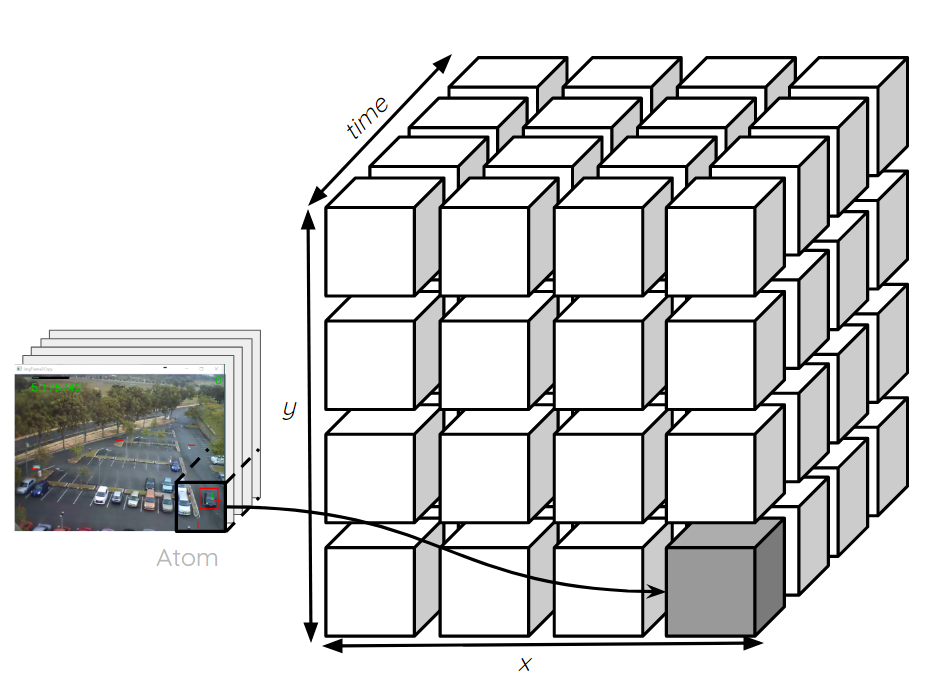
\includegraphics[width=0.6\textwidth]{image/general/atom.PNG}
\caption[Quantization of Video Data into Atoms.]
{Quantization of Video Data into Atoms.
Inspired by the works of \citeA{castanon2016retrieval}.}
\label{fig:atoms}
\end{figure}


In order to design a framework for long-term vehicle semantics extraction from video data, this work adopted the concept of \textbf{"atoms"} as coined by \cite{castanon2016retrieval} which enabled quantization of the video input into individual 3D spatial-temporal cuboids. In this work, an atom is defined as a group of cells at a similar spatial location, that spans a certain fixed number of frames; hence forming a spatio-temporal `cuboid'.
As described in Section \ref{section:dataset_used}, the input video data has a resolution of 640$\times$480 pixels and frame rate of 10$fps$, the dimensions of each atom ($\alpha$) were set to $\alpha_{width}=32$ pixels, $\alpha_{height}=24$ pixels and $\alpha_{time}=10$ frames, which represents the temporal duration of one second. The resolution of the atom ($\alpha_{width},\alpha_{height}$) were set such that the video resolution can be uniformly divided by 20 atoms across both its width and height as illustrated in Figure \ref{fig:viewfromcamera}. Using this setup, each individual atom can be uniquely identified using the $X, Y$ and $T$ identifiers.


However, as mentioned in Section \ref{subsec:vehiclemotionextraction}, the downside of this method is that the accuracy of data representation heavily relies on the number of spatio-temporal cuboids used. With that consideration, the atom's width and height ($\alpha_{width}, \alpha_{height}$) were selected such that one and only one vehicle can occupy a single atom block at any given time. Hence, the colour and trajectory semantics of the vehicles can be adequately represented. While smaller atoms could be used to accurately capture exact location of the vehicle, the additional atoms would only add towards extra computational power needed to process the queries which will be discussed in Chapter \ref{section:retrievalengine}.

The use of these atom-based spatial-temporal cuboids is paramount in this work. By applying the quantization on all axis, the atom-based structure enables two major types of queries to be performed conveniently. Figure \ref{fig:typesofQuery} illustrates the types of queries which are regularly desired when working with video data: \textit{Region of Interest (ROI) query} \& \textit{Time-slicing query}. Typically, the queries used in real world applications are in the form of a combination of both the ROI and time-slicing query where the users are interested in certain activity that occurred in a particular location within a time frame.




\begin{figure}[htb!]
  \centering


\begin{tabular}{cc}
 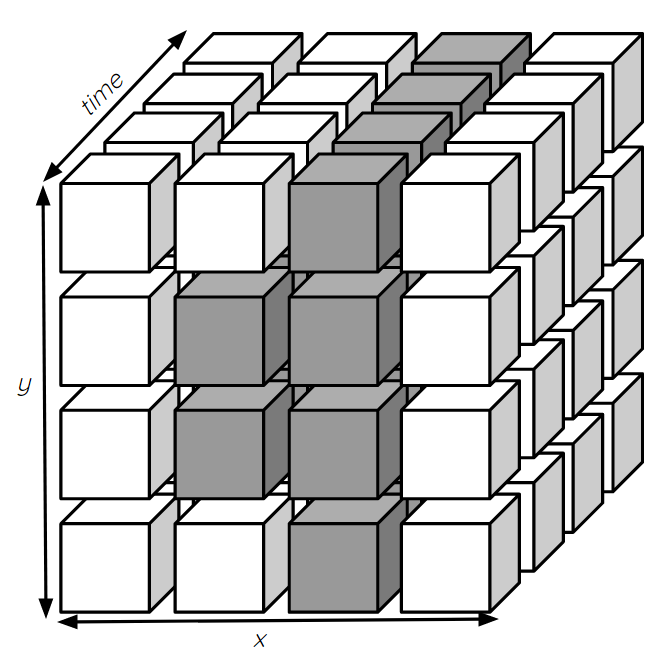
\includegraphics[width=0.3\linewidth]{image/general/atom_ROI.PNG} &  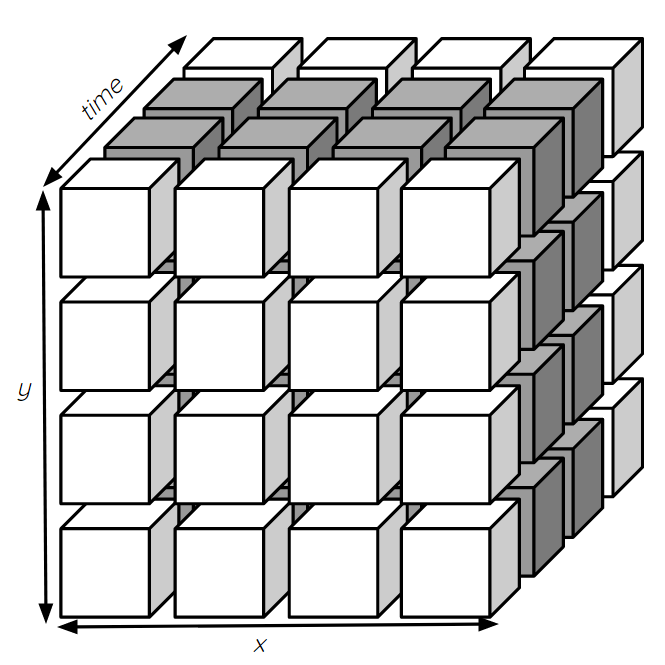
\includegraphics[width=0.3\linewidth]{image/general/atom_time_slicing.PNG}\\
(a) Region of Interest & (b) Time Slicing
\end{tabular}


\caption{Types of Queries} \label{fig:typesofQuery}
\end{figure}



\section{Vehicle Blobs Extraction}
\label{subsection:fundamental}

As described in Section \ref{subsec:scope}, this work assumes that the preliminary task of detecting, tracking and identifying bounding box of each vehicle is obtained prior to the semantic extraction task. This section briefly describes the steps taken by \citeA{lim2017} to detect and extract moving objects in a video using background subtraction techniques to differentiate between static background and moving objects as depicted in Figure \ref{fig:bgs}.

\begin{figure}[htb!]
  \centering
\begin{tabular}{cc}
 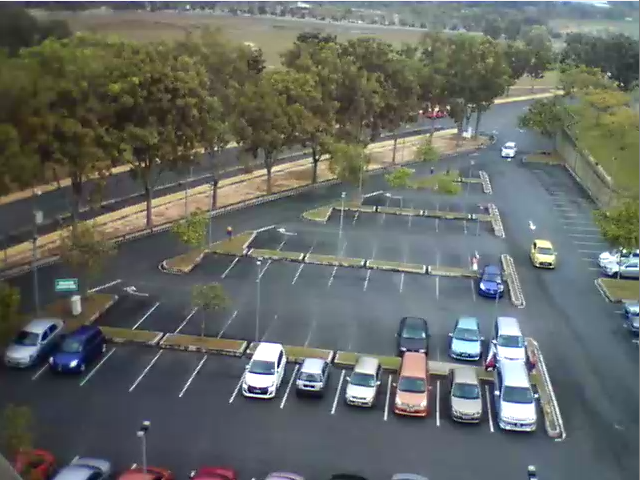
\includegraphics[width=0.4\linewidth]{image/general/bgs1.png} &  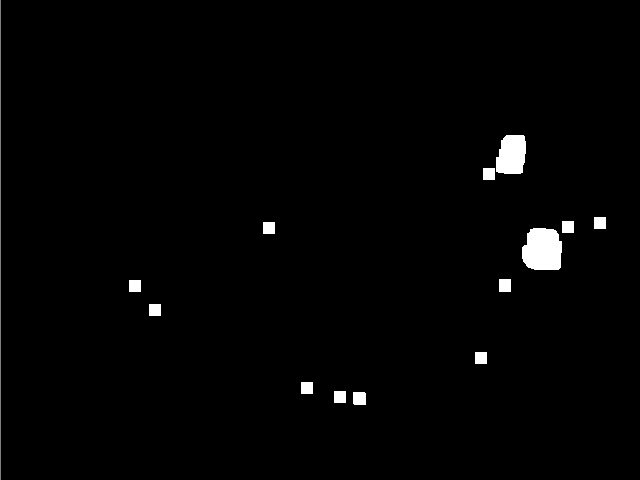
\includegraphics[width=0.4\linewidth]{image/general/bgs2.png}  \\
(a) 123th frame of a video & (b) Result of background subtraction \\
\end{tabular}
\caption{Background Subtraction}
\label{fig:bgs}
\end{figure}

As the vanilla application of background subtraction (BGS) often results with noisy output, the proposed algorithm used in \cite{lim2017} implemented a combination of adaptive learning and frame differencing method. The BGS step was used to detect and extract moving objects (foreground blobs). Several erosion and dilation morphology operations were then performed to further reduce noise and to provide a better representation of foreground blob at the end of the process.
To further improve the accuracy of the extracted blobs, some handcrafted parameters were used to differentiate between vehicles and non-vehicles objects. Furthermore, a deep learning model was deployed to increase the probability of filtering non-vehicle blobs.


\begin{comment}
\begin{figure}[htb!]
  \centering
\begin{tabular}{ccc}
 
\includegraphics[width=0.2\linewidth]{image/general/morph_ori.png} &  
\includegraphics[width=0.2\linewidth]{image/general/morph_erode.png} &
 \includegraphics[width=0.2\linewidth]{image/general/morph_dilate.png}\\
(a) Original Image & (b) Eroded Image & (c) Dilated Image \\
\end{tabular}
\caption{Morphology Operations: Erosion \& Dilation}
\label{fig:morph}
\end{figure}

The process is known as \textit{Opening} occurs when the morphology operations are done in the following sequence - 1) Erosion, \& 2) Dilation, noisy data from the background subtraction method can be eliminated as the erosion operation will be able to remove noise while maintaining the important subjects. In contrast, the operation known as \textit{closing} occurs when the dilation step is first performed, followed by the erosion step. This process is useful to fill up the gaps within the foreground objects. These processes are illustrated in Figure \ref{fig:morph2}

\begin{figure}[htb!]
  \centering
\begin{tabular}{cc}
 \includegraphics[width=0.4\linewidth]{image/general/opening.png} &  \includegraphics[width=0.4\linewidth]{image/general/closing.png}  \\
(a) Opening & (b) Closing \\
\end{tabular}
\caption{Morphology Operations: Opening \& Closing}
\label{fig:morph2}
\end{figure}


\cc{do i need to cite these images? \\}
%https://docs.opencv.org/3.0-beta/doc/py_tutorials/py_imgproc/py_morphological_ops/py_morphological_ops.html
\end{comment}


The work of \citeA{redmon2016you} namely YOLOv2 (You Only Look Once) - a deep learning model was deployed as a complementary module. YOLOv2 is a \textbf{real-time} object detection deep learning model, as the detection process incurred very little overhead to the overall computational time and cost.
With the obtained bounding box, each of foreground blobs were used as an input for the YOLOv2 network. The network will then divide the input into multiple smaller regions and perform prediction of the bounding box along with the class probability. As the YOLOv2 model is pre-trained with vehicles as one of the many classes, no further retraining was done. The tracking of the blobs only took place if they were identified as vehicles. These bounding boxes were then fed into the proposed semantic extraction framework for further processing.


\section{Semantic Extraction}
\label{section:semanticsExtraction}

The ability to extract object specific semantics from the scene is able to provide deeper insights for surveillance purposes.

As describe in Section \ref{subsec:scope}, the two major semantics extracted in the proposed algorithm are (i) \textbf{Vehicle Colour} and (ii) \textbf{Vehicle Trajectory}. Other semantic information such as the time and date which were extracted is briefly discussed as these are simple extraction based on the input file names.
Table \ref{table:semantics} provides a list of all the extracted semantics in this work.
In the following subsections, focus is placed on both the colour and motion semantics extraction process and framework.



\begin{table} \centering
\caption {Types of Extracted Semantics and Methods}
\label{table:semantics}
\begin{tabular}{|l|l|l|}
\hline
\textbf{No.} & \textbf{Semantics Type} & \textbf{Method(s)}                                                                                                          \\ \hline
\textbf{1}   & Date                    & Filename data extraction                                                                                                         \\ \hline
\textbf{2}   & Time                    & Filename data extraction                                                                                                         \\ \hline
\textbf{3}   & Colour                   & \begin{tabular}[c]{@{}l@{}}i) Handcrafted Feature \& Distance Estimation (HSV)\\ ii) Distance Estimation (CIELUV)\end{tabular} \\ \hline
\textbf{4}   & Motion                  & \begin{tabular}[c]{@{}l@{}}i) Handcrafted Feature\\ ii) Collection of Centroid \end{tabular}                                \\ \hline
\textbf{5}   & Object Type             & YOLOv2 (described in \ref{objecttype})                                                                                                               \\ \hline
\textbf{6}   & Size                    & Bounding box from Background Subtraction                                                                                                      \\ \hline
\end{tabular}

\end{table}

\subsection{Colour Semantic}
\label{subsec:colorsemantics}

Without a doubt, colour information plays a significant role as a useful semantics as it is often one of the most common information provided by users when tasked to describe objects from a given event in a particular scene.
However, the process of extracting colour information from vehicles accurately is extremely challenging, especially in an outdoor setting. Often, the white balance of the said scene appears differently depending on various factors such as the ambient illumination during the different hours of the day coupled with weather conditions such as cloudy, rainy or sunshine that may affect the overall scene.
Several commercially available product such as 'Nix colour sensor' \cite{nixsensorltd} and 'Adafruit RGB sensor' \cite{adafruit} makes use of an independent calibrated light source as a means to tackle this challenge.

While colour terms are commonly derived from the Munsell Colour system, there are myriads of available colour terms used in different standards as described in Section \ref{section:colourterm}.
This creates a whole lot of problem in the computing field as colour terms are often described with differing definitions and tuple values.
Hence, there is a dire need of determining the best way to extract and represent colour values with its corresponding colour terms.
Inspirations and ideologies were drawn from the Munsell Colour system and applied in this work.
Although the Munsell Colour system provided a significant research contribution for colour terms naming, the irregularity along the chroma and value axis does not translate well in a modern colour space as the modern colour spaces are often uniformly distributed along all axis.

Hence, in order to better represent the colour space, this work used the Hue-Saturation-Value (HSV) colour space for the colour extraction framework.
The use of the HSV colour space is twofold: Firstly, as the HSV colour space closely resembles the Munsell Colour System, it eases the the colour representation.
Secondly the distance between two colours are now intuitive and linear.
In addition, as HSV colour space is commonly used, the conversion between the RGB and HSV colour spaces are seamless and can be easily introduced into the existing framework. Figure \ref{fig:hsvcylinder} provides a visual representation of the HSV colour space.

\begin{figure}[hbt!]\centering
\includegraphics[width=.5\textwidth]{image/general/HSV.png}
\caption{Hue-Saturation-Value (HSV) Cylinder Visualisation}
\label{fig:hsvcylinder}
\end{figure}

Table \ref{table:allcolourterms} lists several famous web colour dictionary along with the number of colour categories available in each of those colour standards. With so many different colour categories, this ultimately leads to the question of "\textit{How many colour categories should be extracted for the colour semantic? And why?}".
Hence, in this work, the eleven basic colour terms in English proposed by \cite{berlinandkay} was adopted.
\citeA{berlinandkay}'s linguistic approach towards the colour terms assures us that these 11 terms sufficiently describes colours which are often used.
However, the definition of colour terms by themselves are insufficient as it invokes another set of challenge - that is, the representation of these colours in \textit{numerical tuples}, such as RGB values which are typically used in computers.
Linking back to the disccusion in Section \ref{section:eyes}, each and every person has a relatively different perception of colour due to the number of cones cells in the retina. This, compounded with the fact that most monitor screens are not colour calibrated professionally provided an opportunity for Munroe \cite{munroe2010color} to perform an internet crowd-sourcing survey on colour terms and their respective numeral representation according to how colours are displayed on typical monitors.

In \citeA{munroe2010color}'s experiments, 222,500 user sessions consisting of 40,000 women and 100,000 men, provided over five million colours according to their respective colour terms. With the collected results, Munroe then proceeds to map RGB tuples to particular colour terms according to the highest response frequency.
According to Munroe, the mapping of these terms were done by averaging results of several stochastic hill climbing algorithms. At the end of the experiment, 954 colour terms were assigned to a set of RGB tuples of equal size. Figure \ref{fig:xkcd} shows the mapping of dominant colour terms over three fully saturated faces of the RGB cube.
Now, by combining the work of Berlin and Kay along with the work of Munroe, the eleven basic colour terms can now be translated into modern colour tuples using the information collected. These colour terms and the corresponding HEX values are listed in Table \ref{table:colorshex} and these values were treated as \textit{ground truth} for each colour term.
The details of the techniques used in the semantics extraction process in Phase 1 and Phase 2 will be discussed further in the subsequent sections.

\begin{figure}[!hbt]\centering
\includegraphics[width=.6\textwidth]{image/general/xkcd.png}
\caption{Dominant Colour Terms over Three Fully Saturated Faces of the RGB Cube}
\label{fig:xkcd}
\end{figure}


% Please add the following required packages to your document preamble:
% \usepackage[table,xcdraw]{xcolor}
% If you use beamer only pass "xcolor=table" option, i.e. \documentclass[xcolor=table]{beamer}
\begin{table}[!ht]\centering
\begin{tabular}{lcccc}
\cline{2-4}
\multicolumn{1}{l|}{}                     & \multicolumn{1}{l|}{\cellcolor[HTML]{000000}} & \multicolumn{1}{l|}{\cellcolor[HTML]{FFFFFF}} & \multicolumn{1}{l|}{\cellcolor[HTML]{929591}} &                                               \\ \cline{1-4}
\multicolumn{1}{|l|}{\textbf{HEX}}        & \multicolumn{1}{c|}{\#000000}                 & \multicolumn{1}{c|}{\#ffffff}                 & \multicolumn{1}{c|}{\#929591}                 &                                               \\ \cline{1-4}
\multicolumn{1}{|l|}{\textbf{Color Term}} & \multicolumn{1}{c|}{Black}                    & \multicolumn{1}{c|}{White}                    & \multicolumn{1}{c|}{Gray}                     &                                               \\ \cline{1-4}
                                          & \multicolumn{1}{l}{}                          & \multicolumn{1}{l}{}                          & \multicolumn{1}{l}{}                          &                                               \\ \cline{2-5}
\multicolumn{1}{l|}{}                     & \multicolumn{1}{l|}{\cellcolor[HTML]{653700}} & \multicolumn{1}{l|}{\cellcolor[HTML]{E50000}} & \multicolumn{1}{l|}{\cellcolor[HTML]{F97306}} & \multicolumn{1}{l|}{\cellcolor[HTML]{FFFF14}} \\ \hline
\multicolumn{1}{|l|}{\textbf{HEX}}        & \multicolumn{1}{c|}{\#653700}                 & \multicolumn{1}{c|}{\#e50000}                 & \multicolumn{1}{c|}{\#f97306}                 & \multicolumn{1}{c|}{\#ffff14}                 \\ \hline
\multicolumn{1}{|l|}{\textbf{Color Term}} & \multicolumn{1}{c|}{Brown}                    & \multicolumn{1}{c|}{Red}                      & \multicolumn{1}{c|}{Orange}                   & \multicolumn{1}{c|}{Yellow}                   \\ \hline
                                          & \multicolumn{1}{l}{}                          & \multicolumn{1}{l}{}                          & \multicolumn{1}{l}{}                          &                                               \\ \cline{2-5}
\multicolumn{1}{l|}{}                     & \multicolumn{1}{l|}{\cellcolor[HTML]{7E1E9C}} & \multicolumn{1}{l|}{\cellcolor[HTML]{15B01A}} & \multicolumn{1}{l|}{\cellcolor[HTML]{0343DF}} & \multicolumn{1}{l|}{\cellcolor[HTML]{FF81C0}} \\ \hline
\multicolumn{1}{|l|}{\textbf{HEX}}        & \multicolumn{1}{c|}{\#7e1e9c}                 & \multicolumn{1}{c|}{\#15b01a}                 & \multicolumn{1}{c|}{\#0343df}                 & \multicolumn{1}{c|}{\#ff81c0}                 \\ \hline
\multicolumn{1}{|l|}{\textbf{Colour Term}}  & \multicolumn{1}{c|}{Purple}                   & \multicolumn{1}{c|}{Green}                    & \multicolumn{1}{c|}{Blue}                     & \multicolumn{1}{c|}{Pink}                     \\ \hline
\end{tabular}
\caption{Colour Terms and the Corresponding HEX value}
\label{table:colorshex}
\end{table}



\subsection{Motion Semantic}

Without a doubt, the use of video data for surveillance purposes lies in its ability to capture motion information. When tasked to describe an action that occured in a given surveillance setting, signs of motion are usually key information provided by users. In this work, the collective motion performed by a vehicle in the scene is defined as a vehicle's trajectory.

Typically, when describing an event, end user uses a combination of several information such as time of occurrence, description of the objects involved, location and the motion occurred. Traditionally, motion information from videos are converted into text based descriptions using handcrafted methods. For instance, an event such as "\textit{A yellow vehicle was turning into the cross section between Road Alpha and Road Beta at 3:30pm when a black vehicle came rushing over and hitting a pedestrian in the process during commotion}" could be converted into a keyword-based statements such as "yellow car turn left Road Alpha and Road Beta".

However, keyword-based statements are not intuitive and easily interpretable for users who are not familiar with the terminology used in the system.
Futhermore, \cite{bhaumik2016hybrid} claims that the use of textual queries has been proven to be ineffective in video retrieval systems because keywords may not be able to capture the type of semantic content required by an end user.
While motions are not as subjective as the concept of colours, text based descriptions of motion events are less intuitive when compared to a graphical description.
Hence, this work aims to extract motion information such that it can be represented using a graphical form, with the goal of providing a naturally more intuitive representation of a given event.

In the case of a car park scene, the trajectory information from each vehicle is important as it can be used to describes events within the scene.
Hence, it is paramount to ensure motion information from each vehicle is captured and stored accurately.
Given that the types of motion performed in a car park setting varies from user to user, these information were broken into smaller motion information and stored into the database instead of generating a fine representation of motions using conventional motion vector. Both the proposed motion semantics extraction techniques employs different extraction methods which would be discussed further in this chapter.

\subsection{Other Semantic}

In this subsection, the extraction process of the other semantics are briefly discussed. These other extracted semantics includes the time and date information, object type as well as object size. As the extractions of these semantics were simple and/or played little-to-no roles in the both the extraction module and retrieval techniques, the extraction process are described here.

\subsubsection{Date \& Time}

Both date and time information are valuable information in a surveillance setting. In the context of retrieval techniques, these information can be used to narrow down and filter out irrelavent footage. In this work, the camera was set to name the recorded files according to the time and date during the dataset collection process. As the filename contains both the time and date information, the date information can be easily extracted while the time information from frame $\mathbb{T}$ can be deduced when a vehicle is observed in the car park scene as follow:
\begin{align}
    \mathbb{T}_{time}  = (\mathbb{VD} \times \frac{\mathbb{T}}{\mathbb{TF}}) + \mathbb{F}_{time}
\end{align}
where $\mathbb{VD}$ corresponds to the video duration of each file (6 minutes) and $\mathbb{TF}$ is the total frames of the current video. The $\mathbb{F}_{time}$ is the time information extracted from the last six digits of filename, excluding the file extension (see Section \ref{section:dataset_used} for more details). Upon extracting these information, simple formatting is done to ensure these information conform to the typical SQL database requirements.


\subsubsection{Object Type \& Size}
\label{objecttype}
Since the object of interest in this work are the vehicles in the car park scene, YOLOv2 was used to assist the validation of the foreground object detected by the BGS method described in Section \ref{subsection:fundamental}. Objects which were returned under the "vehicle" class were tracked are written into the database. As for the object size, the size of the foreground objects' bounding box were saved in the database as the object size.


\section{\versionOneExt }
\label{section:semantic_lsh}

\subsection{Overview}
Before diving deeper into the nitty-gritty of the \versionOneExt, first, the term Locality Sensitive Hashing needs to be addressed. LSH is a technique used for its ability in dimensionality reduction, this technique excels especially when working with high dimensional data such video data.
This is done by hashing documents with similar properties, mapping and clustering them into a similar neighbourhood. Hence, reducing the dimensionality of a large document in the process. Figure \ref{fig:lshexample} visualises this process.

However, LSH techniques were not implemented in this work. Instead, inspirations to cluster documents with similar properties were drawn from the technique and applied in this work.
In the \versionOneExt, each of the extracted semantics from the vehicles are treated like documents that needs to be  clustered. For the purpose of this work, a total of 11 colour semantic clusters as well as 9 motion semantic clusters were assigned, these clusters were represented using an SQL table individually.
During the semantics extraction process, each of these extracted semantics will then be clustered into these tables according to the colour and motion semantic cluster group.



\begin{figure}[hbt!]\centering
\includegraphics[width=.7\textwidth]{image/new/lsh.png}
\caption{Locality Sensitive Hashing - Documents with similar properties within the dataset are clustered into similar neighbourhood using LSH via the hashing function, h(x). In this example, shapes and colours are used to illustrate documents with similar properties.}
\label{fig:lshexample}
\end{figure}



\subsection{Colour Semantic Extraction }
\label{section:versionOneColorExtract}
%With that in place, this setting effectively performs quantize the range of colours to a fixed number of colour categories while taking advantage of the atom-based structure (Refer to Section \ref{SemanticSegmentation}).

As the background subtraction module has separated the foreground blobs from background scene, these blobs are now assigned a bounding box using the blob's maximum and minimum value on both axis. These bounding box are used to mark the location of the vehicle when a vehicle is detected in the scene. However, due to the background subtraction method adopted, the final foreground blob tend to appear somewhat larger than the actual vehicle footprint.

In order to minimise noise from the bounding box and to obtain a closer estimation of the vehicle's dominant colour, the bounding box is cropped by a factor of 30\% to reduce background noise such as the tar road or vehicles close to it. In order to maintain as much information, the bounding box was not reduced further as that often results in the cropping of the vehicle's windscreen and window regions, thus altering the overall dominant colour.

Upon having the bounding box of the vehicles cropped, the next strategy implemented was to determine the dominant colour of each vehicle by first distinguishing between chromatic and achromatic vehicles. Following similar definition of achromatic colours from Munsell, achromatic colours also known as neutral colours are characterised by the lack of strong hue or chroma values such as black, white and gray colour.

\begin{figure}[htb!]
  \centering
\begin{tabular}{c}
 \includegraphics[width=0.7\linewidth]{image/retrievalOne/all.png} \\
\end{tabular}
\caption{960 Allocated Colour Bins} \label{fig:hsvAllocated}
\end{figure}

The step to differentiate between chromatic and achromatic vehicles was implemented to overcome the shortcomings of the 960 colour bins proposed for the Colour Term Extraction process. Figure \ref{fig:hsvAllocated} illustrates the colour bins generated, the details on how these colour bins were allocated are discussed later. One of the main drawback of the proposed method was the number of bins used to represent the achromatic colours. From the figure, it is observed that while there are a substantial amount of bins representing the almost-pure-black darker tonnes. However, the number of bins used to represent the lighter shades of achromatic colours are just a fraction of the total bins.
This imbalance, compounded with the noise captured (ie: road, other vehicles, trees) during the dominant colour extraction process made it extremely difficult for vehicles to be match with "White" colour term. Hence, this step was introduced as a measure to counterbalance the weakness of the proposed method.


This process of differentiating chromatic against achromatic vehicles starts off by comparing the cropped image, $I_{crop}$, against a grayscale version of the same image, $I_{gray}$. The conversion from RGB to grayscale is performed using $I_{gray} = 0.299 \cdot I_{crop}[R]+0.587 \cdot I_{crop}[G]+0.114 \cdot I_{crop}[B]$. However, as the grayscale image and RGB image does not have the same number of channels, hence, the grayscale image was converted back to a RGB image prior to the comparison.
The absolute difference between these images were obtained using: $I_{Abs_{diff}} = \mid I_{crop} - I_{gray(RGB)} \mid$. Next, the obtained $I_{Abs_{diff}}$ result was subjected to a threshold process for all three channels in the RGB colour space to produce $I_{threshold}(RGB)$.
The step was done to effectively amplify the difference between the original image and the grayscale image, Pixels, $Pv_{(x,y)}$, with values above the threshold value of 35 were set to the maximum value of 255.
\begin{align*}
\label{eq:threshabsolutediff}
I_{threshold}(x,y)(RGB) = \alpha \cdot (255) \\
\text{where, }
\alpha =
\begin{cases}
1, & Pv_{(x,y)} \geq 35\\
0, & otherwise
\end{cases}
\end{align*}

 Finally, the output of the process was converted back to the grayscale colour space to generate $I_{threshold}(gray)$. The hint of significant values at this stage provides an indication of substantial presence of chromatic hues for this particular vehicle.


\begin{comment}
\begin{align}
\label{eq:achromaticSteps}
I_{ori_{i,j}} = \{R_{i,j},G_{i,j},B_{i,j}\} \\
I_{grayscale}, Y_{i,j} = 0.299 \cdot I_{ori}R_{(x_i,y_j)}+0.587 \cdot I_{ori}G_{(x_i,y_j)}+0.114 \cdot I_{ori}B_{(x_i,y_j)}\\
I_{grayscale(RGB_{i,j})} = \begin{cases}R = Y_{i,j}\\G = Y_{i,j} \\ B = Y_{i,j} \end{cases}\\
Abs_{diff}(R,G,B) = \mid I_{ori} - I_{grayscale(BGR)} \mid \\
Threshold_{Abs_{diff}}, T_{Abs_{diff}} =
\begin{cases}R = \begin{cases}Abs_{diff}R\geq 35, & R =255\\ otherwise, & R =0
\end{cases} \\
G = \begin{cases}Abs_{diff}G\geq 35, & G =255\\ otherwise, & G =0
\end{cases} \\
B = \begin{cases}Abs_{diff}B\geq 35, & B =255\\ otherwise, & B =0
\end{cases}
\end{cases}\\
Threshold_{Abs_{diff(grayscale)}} = \\
0.299 \cdot T_{Abs_{diff}}R_{(x_i,y_j)}+0.587 \cdot T_{Abs_{diff}}G_{(x_i,y_j)}+0.114 \cdot T_{Abs_{diff}}B_{(x_i,y_j)}
\end{align}
\end{comment}

With the interest of differentiating between chromatic and achromatic vehicles, the ratio of non-zero pixel value over the total pixels in an image were obtained. This threshold pivot value, $T_{pivot}$, was empirically set at 18\% where vehicles blobs that exceeds this value were assumed to contain strong chromatic hue. The entire process from the original image to the deduction of whether a vehicle blob was chromatic or achromatic is illustrated using Figure \ref{fig:achromatic_thresh}. This handcrafted algorithm allows the deduction of strong chromatic hues and estimates if a particular vehicle blob belongs to a chromatic or achromatic subset.


\begin{figure}[htb!]
  \centering
\begin{tabular}{c}
 \includegraphics[width=0.9\linewidth]{image/general/achromatic_threshold5.PNG} \\
 (a) Achromatic vehicle (Gray/White) \\
 \includegraphics[width=0.9\linewidth]{image/general/achromatic_threshold_color2.PNG}\\
(b) Chromatic vehicle (Red)
\end{tabular}
\caption{(From left) Original image, $I_{crop}$; Grayscale image, $I_{gray}$; Absolute difference, $I_{Abs_{diff}}$; Binary threshold absolute difference, $I_{threshold}(RGB)$; Threshold difference in grayscale, $I_{threshold}(gray)$} \label{fig:achromatic_thresh}
\end{figure}



\paragraph{Achromatic and chromatic colour processing.} Upon determining whether or not the vehicle belongs to the achromatic scale using the $T_{pivot}$ value, the cropped images were then subjected to both the black and white colour filters individually. These simple filters were designed using binary thresholds values empirically set at an intensity levels of 50 and 170 respectively. Next, using a similar fashion, the ratio of non-zero pixels upon filtering were computed. These non-zero percentage ration was used to determine if the vehicle belongs to black, white or gray colour terms. Figure \ref{fig:blackwhite_filter} shows how a white vehicle responds to a black and white filter.


\begin{figure}[htb!]
  \centering
\begin{tabular}{ccc}
 \includegraphics[width=0.22\linewidth]{image/retrievalOne/whitefilter1.png}   &
 \includegraphics[width=0.22\linewidth]{image/retrievalOne/whitefilter2.png}   &
 \includegraphics[width=0.22\linewidth]{image/retrievalOne/whitefilter3.png}   \\
(a) Target Vehicle (White) &
(b) Black Filter Response &
(c) White Filter Response \\
\end{tabular}
\caption{Black \& While Filter Response of a White Vehicle} \label{fig:blackwhite_filter}
\end{figure}




 \begin{algorithm}[!ht]
  \caption{Achromatic Colour Term Extraction}
  \label{algo:achromatic}
  \begin{algorithmic}[1]

  \IF{Percentage of White $>$ 25\%  \\
  \hspace{1em} \&\& Percentage of Black $<$ 25\%}
	\STATE Colour Term = White
  \ELSIF {Percentage of Black $>$ 25\%  \\
  \hspace{1em} \&\& Percentage of White $<$ 25\%}
  	\STATE Colour Term = Black
  \ELSE
  	\STATE Colour Term = Gray
  \ENDIF

  \end{algorithmic}
\end{algorithm}


 \begin{algorithm}[!ht]
  \caption{Colour Term Extraction}
  \label{algo:colorExtract}
  \begin{algorithmic}[1]
    \FOR{Each blob in image}
        \STATE Shrink bounding box \& crop image
        \STATE Create a copy of the cropped image in grayscale
        \STATE Compute absolute difference between cropped image \& grayscale image
        \STATE Perform threshold on absolute difference to amplify difference
        \STATE Convert results into grayscale \& calculate no. of non-zero pixels
            \IF{Ratio of non-zero pixels $>$ $T_{pivot}$}
                \STATE // Chromatic Vehicle
                \STATE Calculate 3D HSV histogram
                \STATE Locate maximum bin location of each channel
                \STATE Map the highest bin from each channel to Colour Term
            \ELSE
                \STATE // Achromatic Vehicle
                \STATE Perform black \& white filter
                \STATE Obtain ratio of non-zero pixels from both filters
                \STATE CALL: Achromatic Colour Term Extraction
            \ENDIF

    \ENDFOR
    \STATE Obtain average dominant colour \& return Colour Term
  \end{algorithmic}
\end{algorithm}


As previously mention, this work chose to primarily work on the HSV colour space, especially for the chromatic colour extraction process. First, the cropped image was converted to the HSV colour space. Then, a 3-Dimensional histogram of the cropped image was generated to identify the maximum value of each channel. However, as colours belongs to a spectrum, using a fine-grained histogram is not ideal as the generated output would be spread across a segment. Hence, the HSV channels were quantized into the following settings: 15 Hue bins, 8 Saturation bins and 8 Value bins for the histogram generation.






% Please add the following required packages to your document preamble:
% \usepackage[table,xcdraw]{xcolor}
% If you use beamer only pass "xcolor=table" option, i.e. \documentclass[xcolor=table]{beamer}
\begin{table}[!ht]\centering
\resizebox{\textwidth}{!}{
\begin{tabular}{c|c|c|c|c|c|c|c|c|c|c|c|}
\cline{2-12}
\multicolumn{1}{l|}{}                        & \multicolumn{11}{c|}{\textbf{Similarity(\%) Based on $D_{Euclidean}$ in HSV Colour Space}}                                                                                                                                                                                       \\ \hline
\multicolumn{1}{|c|}{\textbf{Bin/Colour}} & \textbf{Black} & \textbf{Blue} & \textbf{Brown} & \textbf{Gray}                          & \textbf{Green}                         & \textbf{Orange} & \textbf{Pink}                          & \textbf{Purple}                        & \textbf{Red} & \textbf{White} & \textbf{Yellow} \\ \hline
\multicolumn{1}{|c|}{
\begin{tabular}{c}  \\
\includegraphics[width=0.1\linewidth]{image/HSVcolorspace/img_0_4_7.jpg} \\
\textbf{0, 4, 7}
\end{tabular}     }

& 30.46          & 67.06         & 55.74          & 57.51                                  & 70.94                                  & 73.76           & \cellcolor[HTML]{9AFF99}\textbf{92.18} & 71.95                                  & 72.25        & 64.00          & 76.33           \\ \hline

\multicolumn{1}{|c|}{
\begin{tabular}{c}  \\
\includegraphics[width=0.1\linewidth]{image/HSVcolorspace/img_2_4_3.jpg} \\
\textbf{2, 4, 3}
\end{tabular}     }


& 54.07          & 60.33         & 70.03          & 59.16                                  & 66.14                                  & 55.81           & 64.00                                  & \cellcolor[HTML]{9AFF99}\textbf{81.03} & 59.25        & 49.04          & 55.33           \\ \hline

\multicolumn{1}{|c|}{
\begin{tabular}{c}  \\
\includegraphics[width=0.1\linewidth]{image/HSVcolorspace/img_3_7_4.jpg} \\
\textbf{3, 7, 4}
\end{tabular}     }

& 29.70          & 73.77         & 86.97          & 42.04                                  & \cellcolor[HTML]{9AFF99}\textbf{90.03} & 72.85           & 58.01                                  & 78.43                                  & 76.15        & 33.49          & 72.24           \\ \hline
\multicolumn{1}{|c|}{
\begin{tabular}{c}  \\
\includegraphics[width=0.1\linewidth]{image/HSVcolorspace/img_6_2_6.jpg} \\
\textbf{6, 2, 6}
\end{tabular}     }


& 41.35          & 56.33         & 46.77          & \cellcolor[HTML]{9AFF99}\textbf{75.87} & 62.87                                  & 53.88           & 72.91                                  & 62.49                                  & 52.12        & 69.89          & 58.04           \\ \hline



% ----- remove these?

\multicolumn{1}{|c|}{
\begin{tabular}{c}  \\
\includegraphics[width=0.1\linewidth]{image/HSVcolorspace/img_11_0_0.jpg} \\
\textbf{11, 0, 0}
\end{tabular}     } &

\cellcolor[HTML]{9AFF99}\textbf{88.15} &	21.74 &	35.36 &	60.73 &	31.88 &	17.02 &	34.30 &	41.36 &	19.80 &	39.59 &	17.52
\\ \hline

\multicolumn{1}{|c|}{
\begin{tabular}{c}  \\
\includegraphics[width=0.1\linewidth]{image/HSVcolorspace/img_11_0_1.jpg} \\
\textbf{11, 0, 1}
\end{tabular}     }  &
\cellcolor[HTML]{9AFF99}\textbf{83.66} &	26.71 &	37.51 &	67.13 &	36.19 &	22.35 &	41.39 &	45.70 &	24.80 &	47.38 &	23.04
\\ \hline

\multicolumn{1}{|c|}{
\begin{tabular}{c}  \\
\includegraphics[width=0.1\linewidth]{image/HSVcolorspace/img_11_0_2.jpg} \\
\textbf{11, 0, 2}
\end{tabular}     }  &
\cellcolor[HTML]{9AFF99}\textbf{77.20} &	31.13 &	38.69 &	72.71 &	39.75 &	27.21 &	48.22 &	49.15 &	29.27 &	55.12 &	28.11
\\ \hline

\multicolumn{1}{|c|}{
\begin{tabular}{c}  \\
\includegraphics[width=0.1\linewidth]{image/HSVcolorspace/img_11_0_3.jpg} \\
\textbf{11, 0, 3}
\end{tabular}     }  &
70.02 &	34.87 &	38.85 &	\cellcolor[HTML]{9AFF99}\textbf{76.86} &	42.43 &	31.48 &	54.68 &	51.54 &	33.08 &	62.76 &	32.61
\\ \hline

\multicolumn{1}{|c|}{
\begin{tabular}{c}  \\
\includegraphics[width=0.1\linewidth]{image/HSVcolorspace/img_11_0_4.jpg} \\
\textbf{11, 0, 4}
\end{tabular}     }  &
62.53 &	37.82 &	37.98 &	\cellcolor[HTML]{9AFF99}\textbf{78.73} &	44.10 &	35.06 &	60.60 &	52.69 &	36.13 &	70.25 &	36.44
\\ \hline

\multicolumn{1}{|c|}{
\begin{tabular}{c}  \\
\includegraphics[width=0.1\linewidth]{image/HSVcolorspace/img_11_0_5.jpg} \\
\textbf{11, 0, 5}
\end{tabular}     }  &
54.88 &	39.85 &	36.13 &	\cellcolor[HTML]{9AFF99}\textbf{77.73} &	44.67 &	37.83 &	65.69 &	52.53 &	38.30 &	77.42 &	39.47
\\ \hline

\multicolumn{1}{|c|}{
\begin{tabular}{c}  \\
\includegraphics[width=0.1\linewidth]{image/HSVcolorspace/img_11_0_6.jpg} \\
\textbf{11, 0, 6}
\end{tabular}     }  &
47.14 &	40.88 &	33.38 &	74.20 &	44.10 &	39.67 &	69.54 &	51.05 &	39.50 &	\cellcolor[HTML]{9AFF99}\textbf{83.84} &	41.56
\\ \hline

\multicolumn{1}{|c|}{
\begin{tabular}{c}  \\
\includegraphics[width=0.1\linewidth]{image/HSVcolorspace/img_11_0_7.jpg} \\
\textbf{11, 0, 7}
\end{tabular}     }  &
39.35 &	40.84 &	29.83 &	68.98 &	42.43 &	40.49 &	71.62 &	48.38 &	39.665 &	\cellcolor[HTML]{9AFF99}\textbf{88.23} &	42.61
\\ \hline



% ----- remove these?


\end{tabular}}
\caption{Samples of Similarity Score(\%) based on Euclidean Distance in HSV Colour Space, Highlighted in Green is the Highest Scoring Colour Term}
\label{tab:hsvExample}
\end{table}










This setup ends up with a total of 960 bins where each of these bins are assigned a single colour term based on the closest euclidean distance between this bin's colour and the highest scoring ground truth colour term using the HSV colour space. Using this setup, the colour term which corresponds to the bin(h,s,v) which contains the highest number of hits for a given image is assigned. The examples in Table \ref{tab:hsvExample} shows samples of bins and their corresponding similarity score. However, since the vehicles are moving in the outdoor setting, the ambient and directional lighting (from sun and other light sources) contribute to slight variation of colours. To accommodate the varying lighting condition, the dominant colour of each tracked vehicle from each frame was averaged out throughout its trajectory as illustrated in \ref{fig:ADC}.


As the entire process was done repeatedly over every single frame in the video, the colour term of a particular vehicle is saved into the database while it is tracked. As such, a single vehicle could be classified as a variety of colours depending on the location on where the vehicle was tracked. Algorithm \ref{algo:colorExtract} summarises the strategy used for colour semantic extraction process for the \versionOneExt.



\subsection{Motion Semantic Extraction}
\label{subsec:motions9binextract}

In order to extract motion information of vehicles, the initial step of obtaining the foreground objects from the background subtraction method still stands. Upon identifying these foreground objects, the locations of each vehicles are obtained using the centroids using Equation \ref{eq:centroid}. The motions were extracted by naive position displacement inference methods. Next, the centroids of the vehicles from each frame ($P_N$) are stored in a list, \H{L}.

As two subsequent frames is likely to have too little difference, the algorithm was set to wait until the list has at least 10 records of the previous position before extracting the motion information. Algorithm \ref{algo:motion} provides details of this semantic extraction process in pseudo-code. In this work, the motion of a vehicle is quantized into 8 directional bins (in the form of four cardinal directional and four intermediate directional bins) along with another bin which denotes minuscule and negligible motion information. These quantized directions can be categorised into: UP, DOWN, LEFT, RIGHT, LEFT-UP, LEFT-DOWN, RIGHT-UP, RIGHT-DOWN, MOTIONLESS.

Figure \ref{fig:cardinalbins} illustrates this property. Each of this directions are determined using handcrafted parameters which were selected empirically, the displacement values, $X_{displacement}$ \& $Y_{displacement}$ were set to 5 pixels each. If the difference between the current position of the blob and the position 10 frames ago is larger than either $X_{displacement}$ or $Y_{displacement}$, the motion of the vehicle is updated accordingly. The extracted motion semantic is then saved into the database for each frame.

\begin{figure}[H]\centering
\includegraphics[width=.5\textwidth]{image/new/motion.PNG}
\caption{Directional bins setup}
\label{fig:cardinalbins}
\end{figure}


 \begin{algorithm}[H]
	\caption{Motion Semantic Extraction}
	\label{algo:motion}
	\begin{algorithmic}[1]
		\FOR{Each blob}
		\STATE Save current centroid position ($P_N$) in $List_{motion}$, \H{L}
		\IF{\H{L}.length > 10}
		\STATE Calculate $Difference_x$ and $Difference_y$ using:
		\STATE $Difference_{centroid} = P_N -P_{(N-10)}$
		\IF {Absolute ($Difference_{x}$) > $X_{displacement}$ }
		\IF {$Difference_{x}$ > 0 }
		\STATE Set \textit{Direction(X)} to "LEFT"
		\ELSE
		\STATE Set \textit{Direction(X)} to "RIGHT"
		\ENDIF
		\ENDIF
		\IF {Absolute ($Difference_{y}$) > $Y_{displacement}$ }
		\IF {$Difference_{y}$ > 0 }
		\STATE Set \textit{Direction(Y)} to "UP"
		\ELSE
		\STATE Set \textit{Direction(Y)} to "DOWN"
		\ENDIF
		\ENDIF

		\IF {\textit{Direction(Y)} != NULL AND \textit{Direction(X)} != NULL }
		\STATE Set blob's motion = \textit{Direction(X)} + \textit{Direction(Y)}
		\ELSE
		\IF {\textit{Direction(X)} != NULL }
		\STATE Set blob's motion = \textit{Direction(X) }
		\ELSIF  {\textit{Direction(Y)} != NULL }
		\STATE Set blob's motion = \textit{Direction(Y)}
		\ELSE
		\STATE Set blob's motion = "Motionless"
		\ENDIF
		\ENDIF
		\ENDIF
		\STATE Save blob's current motion into database
		\ENDFOR
	\end{algorithmic}
\end{algorithm}




\section{\versionTwoExt }
\label{section:semantic_chamfer}


\subsection{Overview}

During the course of experimenting with the \versionOneExt, one of the drawbacks identified was that the semantic extraction process was too handcrafted. Although the results could have improved with more tweaking of the parameters and various knobs available, the process of experimenting what works best would be extremely tedious and the end product would not necessarily be extendable to other frameworks depending on the input data.

Along with that, there were several key issues which were identified that could be improved upon. One of the issue pinpointed was that the process of determining whether or not a vehicle belonged to achromatic or chromatic scale was biased. In the dataset on which the experiments were conducted on, there were a lot more achromatic vehicle compared to chromatic vehicle. As the scale was bias, it was easy to manipulate the overall retrieval results by adjusting the parameters to favour the achromatic scale.

The aim of the \versionTwoExt is to provide alternative solutions and improve the performance of the \versionOneExt. In the following subsections, the colour semantic extraction and motion semantic extraction is discussed in detail.



\subsection{Colour Semantic Extraction}
\label{section:versiontwoColor}
As previously discussed in the section \ref{subsec:colorsemantics}, the basic idea of colours is relatively simple for humans, machines on the other hand, have a hard time understanding the concept of colours. In order to extract colour semantics, the initial steps to obtain the Average Dominant colour (ADC) was inherited from the previous method where the bounding box of the detected vehicles from the background subtraction method were cropped.

Next, the dominant colour from each frame was extracted using the maximum bin of the 3-dimension HSV histogram and concatenated. At the end of a vehicle's tracked life cycle, the concatenated dominant colours were averaged out to obtain the ADC. The example in Figure \ref{fig:ADC} illustrates this method while the pseudo-code of the ADC method is described in Algorithm \ref{algo:ADC}.

\begin{figure}[hbt!]\centering
\includegraphics[width=.9\textwidth]{image/general/ADC.png}
\caption{(a) Dominant Colour of the Vehicle at Each Frame; (b) Average Dominant Colour (ADC)}
\label{fig:ADC}
\end{figure}

\begin{algorithm}[H]
  \caption{Average Dominant colour \& Similarity Score Determination}
  \label{algo:ADC}
  \begin{algorithmic}[1]
    \FOR{Each tracked vehicle in the current frame}
        \STATE Shrink bounding box (crop image)
        \STATE Calculate 3D HSV histogram
        \STATE Locate maximum bin location of each channel from histogram
        \STATE Concatenate resulting dominant colours from each frame
        \STATE Obtain the Average Dominant colour (ADC)
        \STATE Measure the difference between ground truth value (Table \ref{table:colorshex}) and ADC
        \STATE Obtain Similarity Score of colour tuple against colour terms
    \ENDFOR
  \end{algorithmic}
\end{algorithm}

In order to reduce the number of parameters and steer clear of handcrafted features such as the one introduced in the previous subsections, instead of assigning one single colour term for each extracted, the similarity score for each colour against all eleven ground truth colours were measured and saved into the database instead. The metrics used to measure the similarity scores between the colours were adopted from the work of Riemersma\cite{riemersma}. This metrics is a low cost estimation of the differences of colours in the LUV linear colour space using RGB values. As the Average Dominant colour was obtained in the HSV colour space, a quick conversion from HSV to RGB colour space was done using Equation \ref{eq:RGBHSVconversion1} to \ref{eq:RGBHSVconversion3}.


%% ---- RGBHSVconversion metric ------------------------------------------------
\begin{equation}
\label{eq:RGBHSVconversion1}
V = \max(R,G,B)
\end{equation}

\begin{equation}
\label{eq:RGBHSVconversion2}
S = \begin{cases}\frac{V - \min(R,G,B)}{V} & , V \neq 0\\
0 & , otherwise \end{cases} \\
\end{equation}

\begin{equation}
\label{eq:RGBHSVconversion3}
H = \begin{cases}
\hspace{2.8em} \frac{60(G-B)}{V-\min(R,G,B)} & ,V = R\\
120 + \frac{60(B-R)}{V-\min(R,G,B)} & ,V = G\\
240 + \frac{60(R-G)}{V-\min(R,G,B)} & ,V = B
\end{cases}
\end{equation}

\centerline{\\$\textit{if } \hspace{.8em}H< 0 \hspace{.8em}\textit{ then } \hspace{.8em}H = H+360.$}





%% ---- RGBHSVconversion metric ------------------------------------------------






According to Riemersma, the benefit of this metrics is that it is a far more stable algorithm where, as quoted, "it does not have a range of colours where it suddenly gives far from optimal results". First, the mean of both the Average Dominant Colour (ADC) and Ground Truth colour (GTC)'s red channel were obtained. Then, this is followed by obtaining the difference, $\Delta$, of all three R, G, and B channels were obtained as well.

In Equation \ref{eq:DiffColorLUV}, the mean of the red channel ($\mean{r}$) is used as a weight for both $\Delta{R}$ and $\Delta{B}$. The details of these equations is described in Equation \ref{eq:RedMeanRGBDiff} and \ref{eq:DiffColorLUV} respectively. Table \ref{tab:luvExample} uses the same example colours as used in Table \ref{tab:hsvExample}, however, the similarity score of the colours were calculated using the metric suggested in Equation \ref{eq:DiffColorLUV} instead of the Euclidean Distance measured in HSV colour space.


%% ---- First metric ------------------------------------------------
\begin{equation}
\begin{split}
\label{eq:RedMeanRGBDiff}
\mean{r} = \frac{C_{1R} + C_{2R}}{2}
\end{split}
% \end{equation}
\quad\quad\quad ; \quad\quad\quad
% \begin{equation}
 \begin{split}
\Delta R = C_{1R} - C_{2R}\\
\Delta G = C_{1G} - C_{2G}\\
\Delta B = C_{1B} - C_{2B}
 \end{split}
\end{equation}

\begin{equation}
\label{eq:DiffColorLUV}
\Delta Colour_{LUV} = \sqrt{(2 + \frac{\mean{r}}{256}) \times \Delta R^{2} + 4 \times \Delta G^{2} + (2 + \frac{255 - \mean{r}}{256}) \times \Delta B^{2} }
\end{equation}




%% ---- First metric ------------------------------------------------



% Please add the following required packages to your document preamble:
% \usepackage[table,xcdraw]{xcolor}
% If you use beamer only pass "xcolor=table" option, i.e. \documentclass[xcolor=table]{beamer}
\begin{table}[!hbt]\centering
\resizebox{\textwidth}{!}{
\begin{tabular}{c|c|c|c|c|c|c|c|c|c|c|c|}
\cline{2-12}
\multicolumn{1}{l|}{}                        & \multicolumn{11}{c|}{\textbf{Similarity(\%) Based on Riemersma's low cost LUV estimation metrics}}                                                                                                                                                                                       \\ \hline
\multicolumn{1}{|c|}{\textbf{Bin/Colour}} & \textbf{Black} & \textbf{Blue} & \textbf{Brown} & \textbf{Gray}                          & \textbf{Green}                         & \textbf{Orange} & \textbf{Pink}                          & \textbf{Purple}                        & \textbf{Red} & \textbf{White} & \textbf{Yellow} \\ \hline
\multicolumn{1}{|c|}{
\begin{tabular}{c}  \\
\includegraphics[width=0.1\linewidth]{image/HSVcolorspace/img_0_4_7.jpg} \\
\textbf{0, 4, 7}
\end{tabular}     }

&
0.00 & 	0.91 & 	28.25 & 	61.27 & 	14.33 & 	67.17 & 	\cellcolor[HTML]{9AFF99}\textbf{70.97} & 	34.74 & 	31.11 & 	25.76 & 	37.78

\\ \hline

\multicolumn{1}{|c|}{
\begin{tabular}{c}  \\
\includegraphics[width=0.1\linewidth]{image/HSVcolorspace/img_2_4_3.jpg} \\
\textbf{2, 4, 3}
\end{tabular}     }


&
34.11 &	22.06 &	\cellcolor[HTML]{9AFF99}\textbf{68.39} &	59.91 &	56.72 &	46.89 &	27.22 &	46.24 &	31.23 &	0.00 &	15.51
\\ \hline

\multicolumn{1}{|c|}{
\begin{tabular}{c}  \\
\includegraphics[width=0.1\linewidth]{image/HSVcolorspace/img_3_7_4.jpg} \\
\textbf{3, 7, 4}
\end{tabular}     }

&
28.13 &	6.53 &	59.41 &	46.70&	\cellcolor[HTML]{9AFF99}\textbf{71.77} &	39.83 &	11.63 &	24.39 &	17.20 &	0.00 &	20.80
\\ \hline
\multicolumn{1}{|c|}{
\begin{tabular}{c}  \\
\includegraphics[width=0.1\linewidth]{image/HSVcolorspace/img_6_2_6.jpg} \\
\textbf{6, 2, 6}
\end{tabular}     }


&
0.00 &	18.72 &	3.55 &	\cellcolor[HTML]{9AFF99}\textbf{70.23} &	27.07 &	16.88 &	44.52 &	18.63 &	0.00 &	46.66 &	27.72
\\ \hline



% ----- remove these?

\multicolumn{1}{|c|}{
\begin{tabular}{c}  \\
\includegraphics[width=0.1\linewidth]{image/HSVcolorspace/img_11_0_0.jpg} \\
\textbf{11, 0, 0}
\end{tabular}     } &

\cellcolor[HTML]{9AFF99}\textbf{89.43}&  	15.88 & 	65.51 & 	10.69 & 	26.97 & 	4.79 & 	0.00& 	35.26 & 	23.58 & 	0.00 & 	0.00
\\ \hline

\multicolumn{1}{|c|}{
\begin{tabular}{c}  \\
\includegraphics[width=0.1\linewidth]{image/HSVcolorspace/img_11_0_1.jpg} \\
\textbf{11, 0, 1}
\end{tabular}     }  &
68.45 &	30.30 &	\cellcolor[HTML]{9AFF99}\textbf{73.87} &	31.62 &	39.47 &	18.66 &	1.26 &	51.17 &	29.17 &	0.00 &	0.00
\\ \hline

\multicolumn{1}{|c|}{
\begin{tabular}{c}  \\
\includegraphics[width=0.1\linewidth]{image/HSVcolorspace/img_11_0_2.jpg} \\
\textbf{11, 0, 2}
\end{tabular}     }  &
47.48 &	39.90 &	\cellcolor[HTML]{9AFF99}\textbf{68.14} &	52.51 &	46.37 &	29.69 &	20.24 &	61.69 &	29.45 &	0.00 &	0.00
\\ \hline

\multicolumn{1}{|c|}{
\begin{tabular}{c}  \\
\includegraphics[width=0.1\linewidth]{image/HSVcolorspace/img_11_0_3.jpg} \\
\textbf{11, 0, 3}
\end{tabular}     }  &
26.52& 	42.30& 	53.27& 	\cellcolor[HTML]{9AFF99}\textbf{73.32}& 	45.52& 	36.31& 	38.11& 	62.02& 	24.32& 	0.14& 	7.44
\\ \hline

\multicolumn{1}{|c|}{
\begin{tabular}{c}  \\
\includegraphics[width=0.1\linewidth]{image/HSVcolorspace/img_11_0_4.jpg} \\
\textbf{11, 0, 4}
\end{tabular}     }  &

5.57 &	36.68 &	35.26 &	\cellcolor[HTML]{9AFF99}\textbf{93.29} &	37.23 &	37.17 &	53.65 &	51.99 &	14.78 &	21.02 &	18.85

\\ \hline

\multicolumn{1}{|c|}{
\begin{tabular}{c}  \\
\includegraphics[width=0.1\linewidth]{image/HSVcolorspace/img_11_0_5.jpg} \\
\textbf{11, 0, 5}
\end{tabular}     }  &

0.00 &	24.52 &	16.04 &	\cellcolor[HTML]{9AFF99}\textbf{83.86} &	23.68 &	32.22 &	64.02 &	36.23 &	2.21 &	42.09 &	26.78

\\ \hline

\multicolumn{1}{|c|}{
\begin{tabular}{c}  \\
\includegraphics[width=0.1\linewidth]{image/HSVcolorspace/img_11_0_6.jpg} \\
\textbf{11, 0, 6}
\end{tabular}     }  &

0.00 &	8.81 &	0.00 &	63.23 &	7.49 &	22.24 &	\cellcolor[HTML]{9AFF99}\textbf{63.64} &	18.07 &	0.00 &	62.88 &	29.66

\\ \hline

\multicolumn{1}{|c|}{
\begin{tabular}{c}  \\
\includegraphics[width=0.1\linewidth]{image/HSVcolorspace/img_11_0_7.jpg} \\
\textbf{11, 0, 7}
\end{tabular}     }  &

0.00 &	0.00 &	0.00 &	42.41 &	0.00 &	8.99 &	53.11 &	0.00 &	0.00 &	\cellcolor[HTML]{9AFF99}\textbf{83.42} &	27.06
\\ \hline



% ----- remove these?


\end{tabular}}
\caption{Samples of Similarity Score(\%) based on Riemersma's low cost LUV estimation metrics, Highlighted in Green is the Highest Scoring colour Term}
\label{tab:luvExample}
\end{table}

The usage of all eleven colour terms to describe an ADC is essential as some colours bears high similarity against the other. A good example would be between pink and red colour; while they are essentially two different colours, however, both these colours belong to a relatively similar hue family. Hence, the similarity score between both these red and pink colour would rather high. This setup allows colours which are visually similar to be ranked higher when the video shots are retrieved using the retrieval engine.

Based on the similarity score (\%) obtained using Riemersma's low cost LUV estimation metrics recorded in Table \ref{tab:luvExample}, the initial analysis of the data shows that distinction between contrasting colour terms are rather clear especially when comparing against the data in Table \ref{tab:hsvExample}.




\begin{figure}[hbt!]\centering
\includegraphics[width=.9\textwidth]{image/analysis/munsell_o.png}
\caption{Munsell 330 Colour Chip}
\label{fig:munsell_ori330}
\end{figure}


\begin{comment}
\begin{figure}[htb!]
  \centering
\begin{tabular}{cc}
 \includegraphics[width=0.45\linewidth]{image/analysis/munsell_a.png}   &
 \includegraphics[width=0.45\linewidth]{image/analysis/munsell_b.png}   \\
(a) Parametric model &
(b) PLSA-individual  \\
 \includegraphics[width=0.45\linewidth]{image/analysis/munsell_e.png}  &
 \includegraphics[width=0.45\linewidth]{image/analysis/munsell_d.png}   \\
(c) Linguistic Approach &
(d) Our method \\
\end{tabular}
\caption[Comparison of the Munsell 330 Colour Chips and the Assigned Colour Terms]{Comparison of the Munsell 330 Colour Chips and the Assigned Colour Terms. (a) Parametric model. Image reproduced from \citeA{benavente2008parametric}; (b) PLSA-individual. Image reproduced from \citeA{van2009learning}; (c) Linguistic Approach. Image reproduced from \citeA{zaslavsky2018efficient}; (d) Proposed Method } \label{fig:munsell_compare}
\end{figure}
\end{comment}



\begin{figure}[htb!]
  \centering
\begin{tabular}{c}
 (a) Parametric model \\
 \includegraphics[width=0.7\linewidth]{image/analysis/munsell_a.png}   \\
 (b) PLSA-individual  \\
 \includegraphics[width=0.7\linewidth]{image/analysis/munsell_b.png}   \\
 (c) Linguistic Approach, Before Compression \\
 \includegraphics[width=0.7\linewidth]{image/analysis/munsell_c.png}   \\
 (d) Linguistic Approach, After Compression \\
 \includegraphics[width=0.7\linewidth]{image/analysis/munsell_e.png}  \\
 (e) Proposed method\\
 \includegraphics[width=0.7\linewidth]{image/analysis/munsell_d.png}   \\
\end{tabular}
\caption[Comparison of the Munsell 330 Colour Chips and the Assigned Colour Terms]{Comparison of the Munsell 330 Colour Chips and the Assigned Colour Terms. (a) Parametric model. Image reproduced from \citeA{benavente2008parametric}; (b) PLSA-individual. Image reproduced from \citeA{van2009learning}; (c, d) Linguistic Approach (Before \& After compression). Image reproduced from \citeA{zaslavsky2018efficient}; (e) Proposed Method } \label{fig:munsell_compare}
\end{figure}


Figure \ref{fig:munsell_ori330} shows the original Munsell 330 Colour chips which contains 10 achromatic colour chips and 320 chromatic colour chips.
The 320 chromatic chips are 40 hues (at full saturation) which are evenly spaced out with 8 different levels of lightness (value) for each hue-value pair (\cite{kay2009world}).
These chips are also known as the World Colour Survey (WCS) stimulus palette.
Figure \ref{fig:munsell_compare} shows the comparison of how the WCS stimulus palette were assigned colour terms using different methods; (a)Parametric model by \citeA{benavente2008parametric}; (b) Probabilistic Latent Semantic Analysis (PLSA) - individual by \citeA{van2009learning}; (c, d) Linguistic and Data Compression approach by \citeA{zaslavsky2018efficient}; (e) Proposed method - which assigns the colour term that contains achieved the highest similarity score (\%) using Riemersma's low cost LUV estimation metrics.

When comparing the parametric model (a) and PLSA model (b) against the linguistic approach (c) and proposed method (e), it is noted that the achromatic tones were given more room to express its nature of low saturation value. However, as the assigning of colour terms are subjective to individuals, is it difficult to measure how well each method performed against each other. Hence, a user study of 77 individuals was conducted to determine which method performed the best to classifying colours from the WCS stimulus into colour terms (Figure \ref{fig:munsell_compare}). The results from the user study is tabulated in Table \ref{tab:munsell_result}.

\begin{table}[H]\centering
\begin{tabular}{|l|c|c|}
\hline
\textbf{Method}                             & \textbf{\# of votes} & \textbf{Percentage (\%)} \\ \hline
(a) Parametric model                        & 17                   & 22.08              \\ \hline
(b) PLSA-individual                         & 20                   & 25.97              \\ \hline
(c) Linguistic Approach, Before Compression & 4                    & 5.19              \\ \hline
(d) Linguistic Approach, After Compression  & 24                   & 31.17              \\ \hline
(e) Proposed method                         & 12                   & 15.58              \\ \hline
\end{tabular}
\caption{User study: Understanding Users' Preference on How Colour Terms Should Be Allocated}
\label{tab:munsell_result}
\end{table}

\vspace{-2em}

While the results tabulated does not favour the proposed method, the overall results shows and agrees with the hypothesis that the division of colour terms according to the colour chips are widely subjective. However, the linguistic approach after compression (d) received the highest number of votes.
However, this approach of testing does not reflect the total capability of the proposed method as the proposed method returns a set of probability for each of the colour terms instead of one final value.



\subsection{Motion Semantic Extraction}
\label{subsec:chamferdistancemotionextraction}

With the intention of extracting motion information from the input video data, the spatio-temporal cuboids or \emph{atoms} were adopted here. Contrary to the framework used in \versionOneExt's motion extraction framework, instead of grouping the motions into 9 directional bins, only the location information of the vehicle is saved. This eliminates the use of handcrafted parameters while maintaining important low level semantics which can be used to represent motion information.


\begin{equation}
\label{eq:centroid}
(Centroid_x, Centroid_y) = (\frac{BB_{x}+BB_{width}}{2} , \frac{BB_{y}+BB_{height}}{2})
\end{equation}
\vspace{-2em}
\begin{align*}
    \text{where BB is the Bounding Box of the vehicle}
\end{align*}

As the background subtraction method has identified the vehicle's location, the centroid of the vehicle can be easily computed by inferring the data from bounding box using Equation \ref{eq:centroid}. Using the \emph{atoms} structure as introduced in Section \ref{section:framework}, each \emph{atom} can be uniquely identified using its' respective identifier via its x, y, and t-coordinate. A vehicle's trajectory, $P$, can be denoted using the collection of  vehicle's centroid from each tracked frame in its life cycle. In this framework, the exact motion of the vehicle held lesser importance when compared to the locality of the vehicle itself.

\begin{align}
    P &= \{ (x_i, y_i, t_i), (x_{i+1}, y_{i+1}, t_{i+1}), (x_{i+2}, y_{i+2}, t_{i+2}), \dotsb,(x_{i+n}, y_{i+n}, t_{i+n})\}  \nonumber \\
      &= \{ t_{p1}, t_{p2}, t_{p3}, \dotsb, t_{pn}\}
\end{align}


Now, in order to determine the motion of the vehicle, the order and sequence of the centroids' t-coordinates was used to represents the motion and the trajectory, $P$, of a vehicle. Figure \ref{fig:motionExample} illustrates the property of this setup which allows trajectories of vehicles to be identified by only using the centroid information. Upon obtaining the location of the centroids, the x \& y-coordinate can be inferred as the atom's width and heights were predefined. Finally, the sequence of the t-coordinate along with the x \& y-coordinates are written into the database as a means of collecting motion information.

\begin{figure}[hbt!]\centering
\includegraphics[width=.9\textwidth]{image/general/trajectorysample2.png}
\caption{Collection of a Vehicle's Centroid to Represent the Vehicle's Motion}
\label{fig:motionExample}
\end{figure}

As a vehicle in the car park scene generally does not move in an irregular motion, the sequence information of the vehicle's centroid holds sufficient clue for the reconstruction and estimation of a vehicle's trajectory within the car park scene. This setup also allows reduction of overhead computational cost and storage space which might occur when converting these centroid information into finer vector features.

\section{Summary}
In this chapter, two different semantic extraction methods were proposed. The semantics that were extracted includes the time date information, colour, motion, object type as well as the size of the objects. Both methods employed a slightly different method of extracting the colour and motion information, the performance of these methods will be discussed in Section \ref{section:retrievalengine}.

For the extraction of vehicle colour semantics, in comparison with the existing methods described in Section \ref{section:litreview}, this work proposed a method that works on videos with relatively low resolution. Next, analysis were done on several colour term mapping methods against the WCS stimulus palette. Given that the mapping of these colour terms is subjective to individual's liking, a user study was perform. The results shows most users prefers the colour model proposed by \citeA{zaslavsky2018efficient} after compression.
In the future, the colour term mapping function can be potentially improved so that the results would resemble the best colour mapping function.


%!TEX ROOT = thesis.tex
\chapter{Semantics Retrieval Engine}
\label{section:retrievalengine}
\section{Introduction}

As described in Section \ref{section:introduction}, there's an evident gap between the process of obtaining user described events and the retrieval of the intended video shots. Traditional approach of collecting text-based description of events alone are insufficient for effective retrieval process.  With the vehicle-specific features such as the vehicle trajectory, time-stamp information, and color information extracted via the extraction module introduced in Chapter \ref{section:semanticsextraction}, retrieval modules were designed to retrieve video shots that resembles user described queries. This chapter aims to engage the topic of semantic retrieval engines in detail and evaluate their performances along with analysis of the end results. 


In this chapter, two retrieval module with relatively different concepts and underlying framework are discussed. The first module was designed with a classic document retrieval system in mind, while the second module was developed in order to address the shortcomings of the first. This is then followed by the methods used to measure the difference between the user-described trajectory, methods used to classify the vehicle color, scoring system along with the results based on multiple user's review of the proposed method. This chapter also includes the speed measurement of the second retrieval engine.

\cc{cc-please measure the VISER retrieval speed and attach the results}


\section{\versionOne}
This section uncovers the techniques used behind the LSH-inspired retrieval engine along with the results.

\cc{write some overview-ish things about this retrieval engine?}

\subsection{Concept}
By taking advantage of the spatio-temporal atom cubes structure introduced in Chapter \ref{section:atoms}, each atom were treated as an unique document. In this setup, each document that contains similar contents were placed in the same SQL table as a mode of clustering documents. An example is given in Table \ref{table:dbSample} to provide a better visualization of the proposed method. These sequence of events is also visualized in Figure \ref{fig:motionExample} with the trajectory marked with \textcircled{2}. 

In the example, a red vehicle was detected frame 180 to 184 of a video file on the 19th of March 2016 at 8:51:00am until 8:51:05am, from atom location (3,15) to (5,17) but was detected as a pink vehicle at frame 181. Using Equation \ref{eq:file_timing}, the event's current frame time can be calculated. Given that the current frame is 181, the current frame time would equate to  $(6_{minutes} \times \frac{181}{360}) + 08:48:00am = 8:51:01am$.

As each cataloged event is treated as a unique document (a single record in the database) in this framework, the retrieval process begins by filtering out tables which are irrelevant to the query. Falling back on the example given in Table \ref{table:dbSample}, the system is able to effectively skip through 9 color tables and 5 motion tables, hence speeding up the process to locate documents of interest while reducing the overhead cost involved when going through an entire database. Upon filtering out irrelevant tables, the retrieval engine proceeds to extract and group all the relevant records according to the filenames. 

Next, the retrieved results are validated to see if they belong to the same vehicle by cross-checking the obj\_id, along with that, the retrieval engine also performs validation to check if the results belong to a similar time-frame by comparing the t-coordinate. This step is essential to ensure that the results belong to the same vehicle trajectory group as the initial tracker may re-assign a obj\_id to another vehicle during the background subtraction process.    


% Please add the following required packages to your document preamble:
% \usepackage[normalem]{ulem}
% \useunder{\uline}{\ul}{}
\begin{table}[!hbt]
\caption{Database structure for a vehicle identified as red and pink color with object id "1" of the \versionOne }
\label{table:dbSample}
\begin{tabular}{llllll}
\multicolumn{6}{l}{{\ul color\_red}} \\ \hline
\multicolumn{1}{|l|}{\textbf{row\_id}} & \multicolumn{1}{l|}{\textbf{filename}}    & \multicolumn{1}{l|}{\textbf{obj\_id}} & \multicolumn{1}{l|}{\textbf{atom\_x}} & \multicolumn{1}{l|}{\textbf{atom\_y}} & \multicolumn{1}{l|}{\textbf{atom\_t}} \\ \hline
\multicolumn{1}{|l|}{n}                & \multicolumn{1}{l|}{20160319\_084800.mp4} & \multicolumn{1}{l|}{1}                & \multicolumn{1}{l|}{3}                & \multicolumn{1}{l|}{15}               & \multicolumn{1}{l|}{180}              \\ \hline
\multicolumn{1}{|l|}{n+1}              & \multicolumn{1}{l|}{20160319\_084800.mp4} & \multicolumn{1}{l|}{1}                & \multicolumn{1}{l|}{3}                & \multicolumn{1}{l|}{16}               & \multicolumn{1}{l|}{182}              \\ \hline
\multicolumn{1}{|l|}{n+2}              & \multicolumn{1}{l|}{20160319\_084800.mp4} & \multicolumn{1}{l|}{1}                & \multicolumn{1}{l|}{4}                & \multicolumn{1}{l|}{16}               & \multicolumn{1}{l|}{183}              \\ \hline
\multicolumn{1}{|l|}{n+3}              & \multicolumn{1}{l|}{20160319\_084800.mp4} & \multicolumn{1}{l|}{1}                & \multicolumn{1}{l|}{5}                & \multicolumn{1}{l|}{17}               & \multicolumn{1}{l|}{184}              \\ \hline
                                       &                                           &                                       &                                       &                                       &                                       \\
\multicolumn{6}{l}{{\ul color\_pink}}                                                                                                                                                                                                              \\ \hline
\multicolumn{1}{|l|}{\textbf{row\_id}} & \multicolumn{1}{l|}{\textbf{filename}}    & \multicolumn{1}{l|}{\textbf{obj\_id}} & \multicolumn{1}{l|}{\textbf{atom\_x}} & \multicolumn{1}{l|}{\textbf{atom\_y}} & \multicolumn{1}{l|}{\textbf{atom\_t}} \\ \hline
\multicolumn{1}{|l|}{m}                & \multicolumn{1}{l|}{20160319\_084800.mp4} & \multicolumn{1}{l|}{1}                & \multicolumn{1}{l|}{3}                & \multicolumn{1}{l|}{16}               & \multicolumn{1}{l|}{181}              \\ \hline
                                       &                                           &                                       &                                       &                                       &                                       \\
\multicolumn{6}{l}{{\ul direction\_down}}                                                                                                                                                                                                          \\ \hline
\multicolumn{1}{|l|}{\textbf{row\_id}} & \multicolumn{1}{l|}{\textbf{filename}}    & \multicolumn{1}{l|}{\textbf{obj\_id}} & \multicolumn{1}{l|}{\textbf{atom\_x}} & \multicolumn{1}{l|}{\textbf{atom\_y}} & \multicolumn{1}{l|}{\textbf{atom\_t}} \\ \hline
\multicolumn{1}{|l|}{h}                & \multicolumn{1}{l|}{20160319\_084800.mp4} & \multicolumn{1}{l|}{1}                & \multicolumn{1}{l|}{3}                & \multicolumn{1}{l|}{15}               & \multicolumn{1}{l|}{181}              \\ \hline
                                       &                                           &                                       &                                       &                                       &                                       \\
\multicolumn{6}{l}{{\ul direction\_motionless}}                                                                                                                                                                                                    \\ \hline
\multicolumn{1}{|l|}{\textbf{row\_id}} & \multicolumn{1}{l|}{\textbf{filename}}    & \multicolumn{1}{l|}{\textbf{obj\_id}} & \multicolumn{1}{l|}{\textbf{atom\_x}} & \multicolumn{1}{l|}{\textbf{atom\_y}} & \multicolumn{1}{l|}{\textbf{atom\_t}} \\ \hline
\multicolumn{1}{|l|}{j}                & \multicolumn{1}{l|}{20160319\_084800.mp4} & \multicolumn{1}{l|}{1}                & \multicolumn{1}{l|}{3}                & \multicolumn{1}{l|}{16}               & \multicolumn{1}{l|}{182}              \\ \hline
                                       &                                           &                                       &                                       &                                       &                                       \\
\multicolumn{6}{l}{{\ul direction\_right}}                                                                                                                                                                                                         \\ \hline
\multicolumn{1}{|l|}{\textbf{row\_id}} & \multicolumn{1}{l|}{\textbf{filename}}    & \multicolumn{1}{l|}{\textbf{obj\_id}} & \multicolumn{1}{l|}{\textbf{atom\_x}} & \multicolumn{1}{l|}{\textbf{atom\_y}} & \multicolumn{1}{l|}{\textbf{atom\_t}} \\ \hline
\multicolumn{1}{|l|}{k}                & \multicolumn{1}{l|}{20160319\_084800.mp4} & \multicolumn{1}{l|}{1}                & \multicolumn{1}{l|}{3}                & \multicolumn{1}{l|}{16}               & \multicolumn{1}{l|}{183}              \\ \hline
                                       &                                           &                                       &                                       &                                       &                                       \\
\multicolumn{6}{l}{{\ul direction\_right\_down}}                                                                                                                                                                                                   \\ \hline
\multicolumn{1}{|l|}{\textbf{row\_id}} & \multicolumn{1}{l|}{\textbf{filename}}    & \multicolumn{1}{l|}{\textbf{obj\_id}} & \multicolumn{1}{l|}{\textbf{atom\_x}} & \multicolumn{1}{l|}{\textbf{atom\_y}} & \multicolumn{1}{l|}{\textbf{atom\_t}} \\ \hline
\multicolumn{1}{|l|}{l}                & \multicolumn{1}{l|}{20160319\_084800.mp4} & \multicolumn{1}{l|}{1}                & \multicolumn{1}{l|}{3}                & \multicolumn{1}{l|}{16}               & \multicolumn{1}{l|}{184}              \\ \hline
\end{tabular}
\end{table}



\subsection{Vehicle Trajectory}
\subsection{Vehicle Color \& Color Mode}

\subsection{Results}



\section{\versionTwo}

\subsection{Concept}
\subsection{Scoring System}
\subsection{Vehicle Trajectory}
\subsection{Vehicle Color \& Color Mode}
\subsection{Results}

\section{Result Analysis}
We also note that the achromatic algorithm is an essential step because the 8 Values bins are insufficient to accurately represent vehicles with borderline dominant color as the brightness values may be widely distributed. 
% js: don't quite understand this
%However, should the initial test against the $T_{pivot}$ fails, the proposed method is able to fall back on the HSV histogram results.

%!TEX ROOT = thesis.tex

\chapter{Conclusion}
\label{section:conclusion}
%\section*{Introduction}

Given that the use of video data as a means of surveillance is a common solution in the our society's yearning for safety and security, there are an abundance of such data sources. However, most of these data are stored unprocessed, and they are only retrieved when an incident dictates the need of doing so. This reactive approach towards an unforeseen event could proved costly to valuable resources such as manpower, time and finance of organisations. The goal of this thesis is to present a preemptive solution towards such incidences by converting large video footages into compact, meaningful semantics which can be retrieved on-the-fly. 

While there has been plenty of works done in the video surveillance domain, only a handful of these works revolve around a car park scenario. Among the existing literature that focused on car park scenarios, a majority of them tend to only focus on detecting the availability of parking spots.
Chapter \ref{section:litreview} provides an overview and critique of recent approaches to extract object semantics such as vehicle colour and motion together with relevant works involving retrieval engines. On a whole, the chapter suggests a considerable room for improvement and research in the field of computer vision and video retrieval for car park surveillance data.
Specifically, this thesis addresses two main objectives: (O1) to extract suitable object semantics that can be easily interpretable while accurately describing scenarios in the car park, and (O2) to retrieve highly relevant (ranked) video footages quickly using a video retrieval engine that is capable of taking in intuitive user-described queries.


%In view of the advantages offered by segmentation of video data, 
The framework used in this work proposed the idea of segmenting input video data into a spatio-temporal cube (\textit{atoms}) structure, similar to that inspired by \cite{castanon2016retrieval}. Different from \cite{castanon2016retrieval}, these \textit{atoms} are used to describe specific locations in a 3D (XYT) space where the extracted vehicle colours and motions are represented. %occurred in both the \versionOneExt and \versionTwoExt modules. 
Besides, this segmentation process also allowed end users to describe trajectories in the form of drawings, which can be intuitively entered into the search canvas. 
The proposed method presented a robust retrieval engine that is able to return a wide range of ranked results without the need for meticulously drawn input trajectory by utilising similarity scores. 
% Methods introduced in both phases: \versionOneRet and \versionTwoRet presented obvious advantages and disadvantages: While the \versionOneRet method was able to accurately pinpoint locations in which an extracted semantic was found, the overall recall rate was significantly lower as the user had to provide very exact queries to retrieve a desired shot. This high accuracy \& low recall rate is useful when the exact query needs to be matched 100\%. 

Overall, the proposed framework and algorithms have been reasonably successful in extracting and retrieving object specific semantics. Given that the trajectory information was stored in a pseudo-Cartesian coordinate manner, the concept used in the proposed method can be extended to various datasets of similar properties. The concluding remarks and future extensions for each of the proposed methods are covered in the following sub-sections.

%\section*{Semantic Extraction, Representation and Retrieval}
\vspace{1em}
\subsection*{Colour Semantic Extraction}
The proposed vehicle colour extraction methods described in Section \ref{section:colourretrieval}  demonstrated robustness over existing handcrafted vehicle colour extraction methods in a low resolution scenario.
By leveraging on the extracted dominant colour of each vehicle over its entire tracked life cycle, the proposed method averaged out the extracted dominant colours to obtain a good estimate of the vehicle's colour.
As such, discoloration due to occlusion and shadows was averaged out as well in the proposed method. Experiments recorded in Chapter \ref{subsec:vehiclecolourchamferdistanceexperiment} showed that the proposed method was able to retrieve vehicle colours accurately: 91\% of the time within the top 3 results.   %While the proposed method might not be able to outperform techniques that apply CNN and SVMs such as those of \cite{hu2015vehicle} (94\%), the proposed method was able to put up a good fight. 
Although the definition of colour terms using the 330 Munsell Colour chips did not favour the proposed method, the adoption of~\citeA{riemersma}'s low cost estimation of difference in colours %in junction with the definition of colours terms 
along with the tuples provided by~\citeA{munroe2010color} proved to be fairly accurate when applied in a retrieval engine setting.     

In the future, the mapping of colour terms can be further improved by clustering the compressed data provided by~\citeA{zaslavsky2018efficient}. Besides, the segmented ROI from the response map of a CNN can also be applied for the extraction of colour information. The experiments in this thesis showed that the use of distance measures to differentiate colours may not be as efficient and accurate when compared to certain deep learning methods. Hence, deep learning models can be explored in the future to improve the classification of these colour terms.

\vspace{1em}
\subsection*{Motion Semantic Representation and Retrieval}
%As dictated in the scope of this work, the bounding box of the vehicles were assumed to be provided. Using the positions of the bounding boxes, the centroid of each box was used to mark the location of the vehicles. 
% In Chapter \ref{subsec:motions9binextract}, the motion information was derived using the previous and current positions of the vehicle. These motion information are then segmented into 9 bins representing various directional categories. While this method provided adequate representation of motion, the hard-coded motion information that was stored beforehand made the retrieval process challenging. Users had to provide the queries accurately to retrieve the desired video footage. At best, the \versionOneRet engine can achieve an accuracy of 95\%, however, at the cost of having to craft input queries very carefully. Also, this proposed method did not show promising recall rates. 

% The drawbacks in \versionOneRet led to the development of \versionTwoRet.
In Chapter \ref{section:motionextraction}, the proposed method suggested that the motion information can be left unprocessed. Instead, the individual location information obtained from the bounding box was represented using spatio-temporal cubes (or \textit{atoms}) can be stored in the database for the retrieval purpose. With this setup, Chamfer Distance was re-purposed as a means to measure the difference between the user's input against the stored data. The retrieval engine presented users with an input canvas where the motion of a desired vehicle could be drawn intuitively at will. The trajectories of the input query were translated from the input sequence information whereby the motion was drawn. The proposed retrieval engine was able to achieve an accuracy of 100\% for the top-3 results based on simple trajectories. However, when presented with complex trajectories that involved multiple turnings, the accuracy dropped to 67\%. Overall, the retrieval engine achieved an average accuracy of 82\% for the top-3 results.

While the proposed retrieval engines were able to successfully retrieve the desired video footages to a good extent, there are still some inherent weaknesses. In terms of increasing its usefulness, the retrieval engine can be extended to retrieve shots containing multiple trajectories. This would be very useful in scenarios involving multiple vehicles such as accidents. Next, the retrieval engine can also be extended to include specific parking spots of the vehicles. In the current setup, the retrieval engine only evaluates the results based on its overall trajectories or movements within the car park. However, in a car park scenario, the parking location of the vehicle should also be considered as an \emph{event} while describing activities in a car park.

\vspace{1em}
\subsection*{Final Remark}
This work done in this thesis has achieved the objectives of identifying and extracting useful object semantics that can accurately describe the events in a car park scenario. A retrieval engine that takes in user-described trajectories along with other object specific semantics such as colour as well as time and date information allows users to easily define the desired queries in a realistic manner. As the retrieval engine was developed using web based technology, it is easy for such systems to be implemented directly on modern web browsers which are fully independent of the underlying Operating System (OS) of the machine. This also allows the results to be retrieved quicker as the resulting videos do not need to be decoded and re-encoded to specific time periods as \emph{HTML5} video supports `Media Fragments URI'. For instance, to play a video from the 10th second to the 20th second, a time parameter (\emph{i.e.} $t=10,20$) can easily specified. While the overall goal of this thesis was achieved, we presented a number of future extensions for the betterment of the proposed system.

\appendix
%!TEX ROOT = thesis.tex
\chapter{Manuals, Technical Specifications, Documentations, Example Scenarios}
%!TEX ROOT = thesis.tex
\chapter{Try}

\lipsum[1-2]

\backmatter
\bibliography{llt}
\printglossaries
\theendnotes
{\SingleSpacing\printindex}

\ownpubs
\nociteconf{cheong2018vehicle,lim2017}
%\nocitejour{Lim:Ranaivo:Tang:Polibits:2011,Lim:Ranaivo:Tang:Procedia:2011}
%\bibliographyjour{llt}
\bibliographyconf{llt}

\end{document}